\documentclass[
  utf8,%     More capable input encoding than latin-1.
  % parskip,%  For vertical whitespace between paragraphs.  This comes down to more than just using parskip.sty, so it's better to use this class option.
  % S5MP % If you intend to really use margin paragraphs (not recommended!).
%  crop,%     Produce output with crop marks and paper size A4.  Liu-Tryck should like this.  Automatically adds information, including the physical page number, at the top of each page.
       %     Add option 'noInfo' to suppress the info at the top of each page when using option 'crop'.
  % Font options: 'kp' (default), 'times', 'lm'.  The KpFonts (loaded using 'kp'), is the most complete font among the provided options.  Among other, it supports slanted small caps.  See rtthesis.cls for more details regarding the font options.
  largesmallcaps,intlimits,widermath,% Good options to KpFonts.
  sharecounter,nobreak,definition=marks,%  See comments in the results chapter of this document for more information on these options!
  numbers, % If you want to cite references by numbers, use this option.
  noparts% Use option 'noparts' if you do not make use of part divisions.
]{rtthesis}

\usepackage{mythesis}

\documentclass{article}

\usepackage[style=ieee,backend=biber]{biblatex}
\addbibresource{./bibtex/bib/cite.bib}


\usepackage[margin=3cm]{geometry}
\usepackage[utf8]{inputenc}
\usepackage{color}
\usepackage{todonotes}
\usepackage{amsmath}
\usepackage{float}
\usepackage{graphicx} % Allow graphics.
\usepackage{csquotes}
\usepackage{tikz} 
\usepackage{nonfloat}
\usepackage[ampersand]{easylist}
\usepackage{pdfpages}
\usepackage{subcaption}
\usepackage{caption}
%\usepackage{subfig}
\usepackage{mathrsfs,amsmath}
\usepackage{fancyhdr}
\usepackage{listings}
\usepackage{placeins}   

\usepackage{amsfonts}
% or
%\usepackage{amssymb}

\usepackage{listings}
\usepackage{color}
 
\definecolor{codegreen}{rgb}{0,0.6,0}
\definecolor{codegray}{rgb}{0.5,0.5,0.5}
\definecolor{codepurple}{rgb}{0.58,0,0.82}
\definecolor{backcolour}{rgb}{0.95,0.95,0.92}
 
\lstdefinestyle{mystyle}{
    backgroundcolor=\color{backcolour},   
    commentstyle=\color{codegreen},
    keywordstyle=\color{magenta},
    numberstyle=\tiny\color{codegray},
    stringstyle=\color{codepurple},
    basicstyle=\footnotesize,
    breakatwhitespace=false,         
    breaklines=true,                 
    captionpos=b,                    
    keepspaces=true,                 
    numbers=left,                    
    numbersep=5pt,                  
    showspaces=false,                
    showstringspaces=false,
    showtabs=false,                  
    tabsize=2
}
 
\lstset{style=mystyle}
 
 
%%
\usepackage{nomencl}
\makenomenclature

%% This removes the main title:
\renewcommand{\nomname}{}
%% this modifies item separation:
\setlength{\nomitemsep}{8pt}
%% this part defines the groups:
%----------------------------------------------
\usepackage{etoolbox}
\renewcommand\nomgroup[1]{%
  \item[\Large\bfseries
  \ifstrequal{#1}{N}{Nomenclature}{%
  \ifstrequal{#1}{A}{List of Abbreviations}{}}%
]\vspace{10pt}} % this is to add vertical space between the groups.
%----------------------------------------------

\usepackage{subcaption}
\begin{document}
\selectlanguage{english}

\frontmatter
\maketitle

\begin{abstract}[swedish]
  Foton tagna i det korta infraröda spektrumet är intressanta i militära sammanhang på grund av att de är mindre beroende av vilken tid på dygnet de är tagna för att solen, månen, stjärnor och nattsken (night glow) lyser upp jorden med kortvågiga infraröd strålning dynget runt. Ett stort problem med dagens kortvågig infraröda kameror är att de är väldigt dyra att producera och därav inte tillgängliga till en bred skara, varken militärt eller civilt. Med hjälp av en relativt ny teknik kallad \textit{compressive sensing} (CS) möjligörs en ny typ av kamera med endast en pixel i sensorn. Denna nya typ av kamera behöver bara en bråkdel mätningar relativt antal pixlar som ska återskapas och reducerar kostnaden på en kortvågig infraröd kamera med en faktor 20. Kameran använder en mikrospegelmatris som används för att välja vilka speglar (pixlar) som ska mätas i scenen och på så sätt skapa ett underbestämt ekvationssystem som kan lösas med teknikerna beskrivna i CS för att återskapa bilden. Givet den nya tekniken är det i Totalförsvarets forskningsinstituts (FOI) intresse att utvärdera potentialen hos en enpixel-kamera. Med en enpixel-kameraarkitektur utvecklad av FOI var målet med detta examensarbete att ta fram metoder för att sampla, återskapa bilder och utvärdera deras kvalitet. Detta examensarbete visar att användning av strukturella slumpade matriser och snabba transformer öppnar upp för högupplösta bilder och snabbar upp processen att rekonstruera bilder avsevärt. Utvärderingen av bilderna kunde göras med vanliga mått associerade med kamerautvärdering och visade att kameran kan återskapa högupplösta bilder med relativt hög bildkvalitet i dagsljus. \citep{article:FOI_pres_sens}
\end{abstract}

\begin{abstract}[english]
  

Photos captured in the shortwave infrared (SWIR) spectrum are interesting in military applications because they are independent of what time of day the picture is captured because the sun, moon, stars and night glow illuminate the earth with short-wave infrared radiation constantly. A major problem with today's SWIR cameras is that they are very expensive to produce and hence not broadly available either within the military or to civilians. Using a relatively new technology called compressive sensing (CS), enables a new type of camera with only a single pixel sensor in the sensor (a SPC). This new type of camera only needs a fraction of measurements relative to the number of pixels to be reconstructed and reduces the cost of a short-wave infrared camera with a factor of 20. The camera uses a micromirror array (DMD) to select which mirrors (pixels) to be measured in the scene, thus creating an underdetermined linear equation system that can be solved using the techniques described in CS to reconstruct the image. Given the new technology, it is in the Swedish Defence Research Agency (FOI) interest to evaluate the potential of a single pixel camera. With a SPC architecture developed by FOI, the goal of this thesis was to develop methods for sampling, reconstructing images and evaluating their quality. This thesis shows that structured random matrices and fast transforms have to be used to enable high resolution images and speed up the process of reconstructing images significantly. The evaluation of the images could be done with standard measurements associated with camera evaluation and showed that the camera can reproduce high resolution images with relative high image quality in daylight.

\end{abstract}

\begin{acknowledgments}
 HELLO

  \addvspace{1em}
  \begin{flushright}
    \textit{%
      Link\"{o}ping, Januari 2018\\
      Andreas Brorsson%
    }
  \end{flushright}
\end{acknowledgments}


\tableofcontents
\begin{notation}% Passing the option "old" to the notation environment will redefine the notationtabular environment so that it produces an old style LaTeX tabular instead of a booktabs.sty style tabular.
  \centering

  \begin{notationtabular}{Nomenclature}{Notation}{Meaning}
    $\mathbf{y}$ & Measured signal \\
    $\mathbf{\Phi}$ & Measurement matrix  \\
    $\mathbf{x}$ & The spatial scene \\
    $\mathbf{\Psi}$ & Basis matrix \\
    $\mathbf{\theta}$ & Coefficients in basis $\Psi$ \\
    $\mathbf{A}$ & Sensing matrix in new basis \\
    $N$ & Number of reconstructed pixels \\
    $M$ & Number of single pixel measurements \\
    $\epsilon$ & Noise from measurements \\
  \end{notationtabular}

  \begin{notationtabular}{Abbreviations}{Abbreviations}{Meaning}
  	\abbrBRISQUE\index{BRISQUE@\abbrBRISQUE!abbreviation} & Blind/referenceless image spatial quality evaluator\\
    \abbrCS\index{CS@\abbrCS!abbreviation} & Compressive sensing \\
    \abbrCI\index{CS@\abbrCI!abbreviation} & Compressive imaging \\
    \abbrDLP\index{DLP@\abbrDLP!abbreviation} & Digital light processor\\
    \abbrDMD\index{DMD@\abbrDMD!abbreviation} & Digital micromirror device\\
    \abbrIID\index{IID@\abbrIID!abbreviation} & Independent and identically distributed \\
    \abbrFOI\index{FOI@\abbrFOI!abbreviation} & Swedish Defence Research Agency \\
    FWHT & Fast Walsh-Hadamard transform \\
    
    PSNR & Peak signal-to-noise ratio \\
    
    	\abbrRIP\index{RIP@\abbrRIP!abbreviation} & Restricted isometry
property\\
	\abbrSLM\index{SLM@\abbrSLM!abbreviation} &  Spatial Light Modulator\\
    \abbrSPC\index{SPC@\abbrSPC!abbreviation} & Single pixel camera\\

    \abbrSRM\index{SRM@\abbrSRM!abbreviation} & Structurally random
matrix\\

	SSIM & Structural similarity\\
	
	\abbrSWIR\index{SWIR@\abbrSWIR!abbreviation} & Short-wavelength infrared\\
	
	\abbrTV\index{TV@\abbrTV!abbreviation} & Total variation\\
	
  \end{notationtabular}
\end{notation}


\mainmatter
\section{Introduction}
The development and research of compressed sensing applied to a single pixel camera (SPC) is a relative new area in signal processing with the first functioning camera architecture in 2006. Since then numerous improvements and methods have been proposed how to capture images. In this section a introduction to the SPC architecture and a brief introduction of compressed imaging is presented followed by the aim, research questions and thesis outline. 

\subsection{Compressive sensing \& imaging}
Compressive sensing is a new sampling strategy which reconstructs a compressible or sparse signal by finding solution to undetermined linear system where the number of measurements $M$ is less then the number of data points $N$ in signal. Two constraints need to be fulfilled to apply compressed sensing sampling: the sampled signal needs to be spares in some basis e.g. Fourier or gradient, the second condition is that the measurement matrix must be incoherent with the sparse transform. The characteristic  undetermined linear system in CS is defined as $ \mathbf{y} = \mathbf{\Phi}\mathbf{x}$ where $\mathbf{y}$ contains the measurements from the measurement matrix $\mathbf{\Phi}$ sensing the signal $\mathbf{x}$. In figure~\ref{fig:CS_eq_sys} such linear equation system is shown.

\begin{figure}[H]
	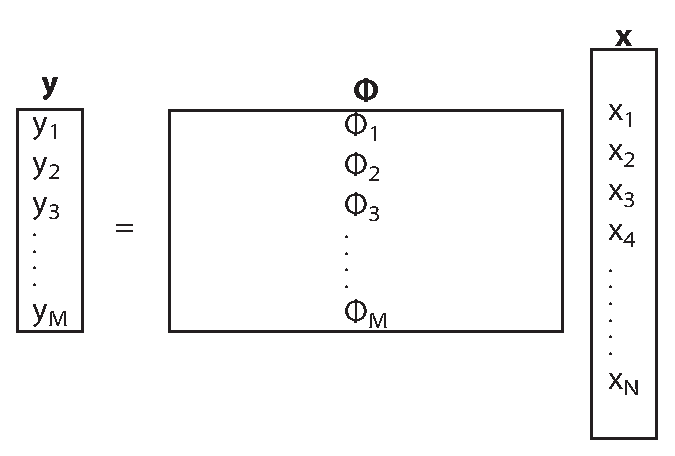
\includegraphics[scale=0.5]{gfx/CS_eq.eps}
	\caption{CS undetermined linear system}
	\label{fig:CS_eq_sys}
\end{figure}



Scientists at Rice university in Texas, USA realized that the new method could be used to create a new camera architecture with a single photo diode in the sensor, the single pixel camera was born and thus a new sub field of compressed sensing was created called compressive imaging.\\[0.1in] 

To be able to apply CS to imaging in the first place the constraints in CS needs to hold for images as well. The first requirement is that the signal needs to be compressible or sparse in some basis which natural images is known to be because they can be compressed using for example JPEG (Descrete cosine transform), JPEG2000 (Wavelet). The second constraint is that the measurement matrix must be incoherent with the sparse transform which for example white noise or some structure with the same property as white noise.\\[0.1in]

\subsection{System architecture}
The SPC in this master's thesis was designed with reflecting telescope optics to act as a lens to focus the scene. As seen in figure~\ref{fig:system_overview} light from the scene enters through the aperture in the camera where the primary mirror focus the light the via the secondary mirror onto the DMD. To this point, the SPC works like a conventional camera with a DMD where the image sensor would be placed in the convectional camera. So the SPC has an digital micromirror array in the focal point which resemble an image sensor but instead of photo diodes for each pixel there is a tiny mirror which individually can ether reflect light 12 degrees to the right or left as seen in figure~\ref{fig:system_overview}. The incomming focused light can ether be dumped or it can be reflected into the single pixel detector through an lens. 


\begin{figure}[H]
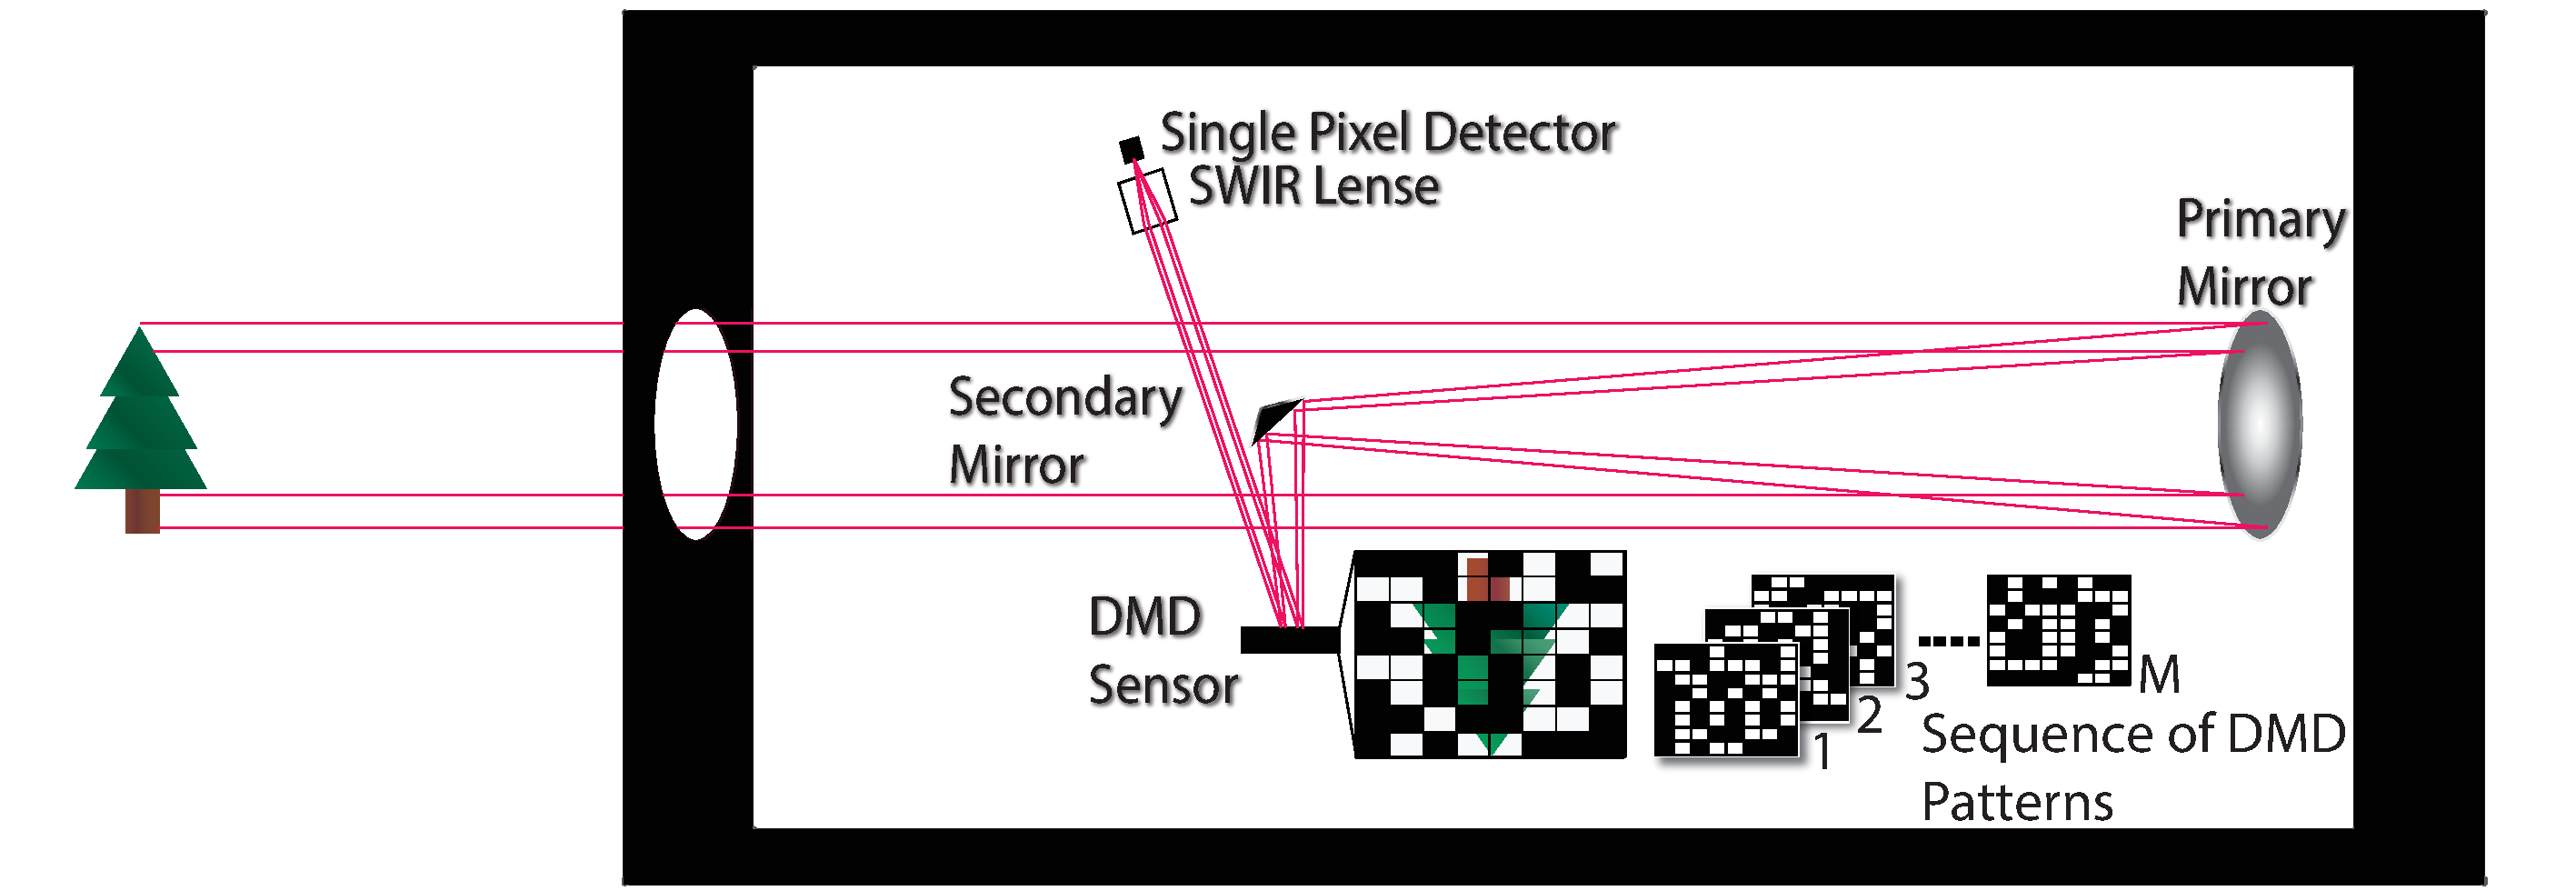
\includegraphics[width = \linewidth]{gfx/System_gif.eps}
	\caption{System overview}
	\label{fig:system_overview}
\end{figure}	

To connect the architecture with the math from CS it can be interpreted as, the light from the scene which is focused on the DMD is the desired signal $\mathbf{x}$, the image. The DMD can individually set each mirror the ether direct the light from each 'pixel' to the single pixel sensor or dump the light i.e a spatial light modulator (SLM). The DMD sets a pattern of pixel of intress which is a measurement matrix $\Phi_m$ to be summarized in the single pixel sensor $y_m$ as a measurement. One measurement is the inner product of a measurement matrix and the signal, $\Phi_m \times x = y_m$. To complete a full measurement the process is repeated with different measurement matrices set on the DMD to the full undetermined linear system $ \mathbf{y} = \mathbf{\Phi}\mathbf{x}$.

\subsection{Measurement matrix \& reconstruction}
How is the measurement matrix chosen? As told before the measurement matrix needs to be incoherent with the sparse transform and the DMD can only direct he light or not which mathematically is ether a zero or a one. The research tells that for example a i.i.d. Gaussian distribution with equal probability of a zero or one will with high probability be incoherent with a natural image scene. But how about the first constraint that the signal $\mathbf{x}$ needs to be sparse or compressible in some basis? Often natural images is not sparse in the spatial domain unless the scene is for example the night sky, well a good property of CS that the scene can be transformed to an other basis like this,

\begin{equation}
\label{eq:CS_1}
\mathbf{y} = \mathbf{\Phi} \mathbf{x} \Leftrightarrow \mathbf{y} = \mathbf{\Phi} \mathbf{\Psi} \mathbf{\Theta},
\end{equation}

where $\mathbf{\Psi}$ is a sparsitfying basis for example to the DCT or Wavelet basis. And $\mathbf{\Theta}$ is the coefficients vector which is more sparse then the spatial coefficent vector $\mathbf{x}$. And the transformation will not comprimize the incoherence between the reconstruction matrix $A = \Psi\Phi$ and the coeficents $\Theta$ in the new basis. This means that the signal $\mathbf{x}$ will be reconstructed with optimization in a more sparse basis $\Theta$ and then transformed back to the spatial domain.\\[0.1in]

What i special about CS is not just how the problem is presented but also how to solve it. It is known that an undetermined linear system as infinite many solution so how does the signal get recovered? CS exploit the characteristics of the signal $x$ which is known to be sparse in some basis. With for example $\ell_1$ optimization,

\begin{equation}
\label{eq:l1_1}
\widehat{\mathbf{\Theta}} = \text{arg min} ||\mathbf{\Theta} ||_{\ell_1} \text{ subject to } \mathbf{\Psi} \mathbf{\Theta} \Theta = y,
\end{equation}    

which means that $\ell_1$ optimization minimizes the non zero elements of $\Theta$ and can exactly reconstruct a K-spares vector or approximate a compressible vector. The exact recovery can be accomplished with high probability using $M \geq \mathcal{O}(K\text{log}(N/K))$ measurements. This is why CS is powerful, it enables sub-Nyquist measurements with exact recovery in the noiseless case which can be approximated in real applications.\\[0.1in]

In the compressed imaging case where noise is present an other optimization algorithm has shown to be more successful at recovering images: total variation. Total variation regularization minimizes the magnitude of the gradient in the image and doing so it preserve edges and piece-wise constant structure in the image which is desired.     

 
\subsection{Motivation}
Why would a SPC be beneficial to a conventional camera? The SPC has more components to work and several measurements have to be made over time while a regular camera measures all pixels on the sensor at the same time and the reconstruction shifts burden to the processor.

\begin{itemize}
\item Why?
\item Compress before the images is taken
\item Cheaper and in some cases only possible case to go to larger resolutions
\item It is more effective then scanning each pixel one by one because the one need to do N samples.
\end{itemize}


\subsection{Aim} 
What image quality can be achieved in natural images captured with a single pixel camera in daylight using state of the art methods?  


\subsection{Research questions} 
\label{sec:RQ}
\begin{itemize}
    \item How can the quality of images reconstructed by CS or a SPC be evaluated?
    \item What is the state of the art method to capture and reconstruct images using a SPC architecture?
    \item What image quality is achieved using state of the art methods applied to the SPC?
\end{itemize}


\subsection{Limitations}
\begin{itemize}
    \item The hardware rig provided by FOI
    \item 
\end{itemize}



\subsection{Thesis outline}

\section{Related work}
In this section important, relevant and fundamental articles to this master's thesis is presented each with a summary. The articles covers compressed sensing theory applied to compressed imaging, SPC architecture and how to evaluate the images i.e. the fundamental source of information on how to build a state of the art SPC system and how to evaluate its performance. 

\subsection{Compressive sensing}
\begin{itemize}


\item \cite{book:sm, book:srr} "Sparse Modeling" by G. Y. Grabarnik and  I. Rish and "Sparse and redundant representation" by M Elad is two books which thoroughly presents the topic of sparse and redundant representation and modeling. The fundamental principles and constraints that needs to be fulfilled in CS. The books presents different minimization algorithms and how to implement them.   

\item In~\cite{article:CS_donoho1} "Compressed sensing" David L. Donoho proposed the framework of compressed sensing and the application of images capturing.

\item \cite{article:CS_from_theory_a_sur} "Compressive Sensing: From Theory to Applications, A survey" by S. Qaisar et al. 2013, reviews CS background, theory and mathematics and has a extensive survey of reconstruction algorithm and potential CS applications.

\end{itemize}
\subsection{Compressive imaging}
\begin{itemize}

\item \cite{article:an_Arcitecture_for_CI,article:a_new_ci_arc} "An architechture for compressive imaging" and "A New compressive imaging camera architecture using Optical-Domain Compression" by M. B. Wakin, D Takhar, et al. 2006, presents the first single pixel camera architecture using CS to reconstruct the images. 

\item \cite{article:single_pixel_im_cs} "Single-Pixel Imaging via Compressive Sampling" by M. F. Duarte et al. 2008, is an introduction and summary to CS and CI including the SPC architecture. This article also compares different scanning methodologies and their conditions.   

\item \cite{article:foiSPIS} "Single Pixel SWIR Imaging using Compressed Sensing" by C. Brännlund and D. Gustafsson. 2016, was written to show the initial results and proof of concept of the SPC architecture at FOI.
  
%\item \cite{article:cs_for_prac_ios_a_tut} "Compressed sensing for practical optical imaging systems: a tutorial"


\item \cite{article:a_high_res_swir} "A high resolution SWIR camera via compressed sensing" is a paper from L. McMackin et al. 2012 at Inveiw Technology which develop and produces compressive sensing cameras. The paper contains a brief review of CS and CI followed by a presentation of their camera architecture. 

 
\item \cite{mt:EF} "Compressed Sensing for 3D Laser Radar" by E. Fall. 2014, is a master's thesis where CS/CI is evaluated for a potential depth camera architecture using a one pixel sensor.   

\item \cite{article:misuperres} "Multi image super resolution using compressed sensing" by T. Edler et al. 2011, presents the results from using a small detector array instead of just one single sensor, but still using CS to reconstruct the images. With this technique the subsampling ratio and the exposure time is reduced. 

 
	
\end{itemize}
    
\subsection{Measurement matrix \& reconstruction}

\begin{itemize}
    
\item \cite{article:TVAL3} Chengbo Li:s master's thesis "An Efficient Algorithm For Total Variation Regularization with Applications to the Single Pixel Camera and Compressive Sensing" describes a total variation algorithm Li constructed which solve the CS problem. The algorithm is faster and produces better results for images than previous popular algorithms.   

\item \cite{article:SRM_short, article:SRM_long, article:SRM_block} Fast and Efficient Compressive Sensing Using Structurally Random Matrices (SRM). The articles describes why and how to implement SRM, in these articles the Hadamard or DCT matrices is proposed to replace the i.i.d random matrix. With SRM the reconstruction time is reduced by replacing matrix multiplication with fast transforms. In addition to improved reconstruction time the new method does not need to store the measurement matrix in memory which enables reconstruction of high resolution images. 

\item \cite{article:an_improved_WH_matrix} "An Improved Hadamard Measurement Matrix Based on Walsh Code For Compressive Sensing" Shows that sequency-ordered Walsh Hadamard matrix gives better reconstruction then the Hadamard matrix with the same benefits of using the Hadamard matrix. The resulting reconstructed image has near optimal reconstruction performance.
	

\end{itemize}


\subsection{Evaluation}

\begin{itemize}

\item \cite{book:image_processing} "The essential guide to image processing" by Al Boviks contains the majority of fundamental image processing techniques and measurements. Two image quality metrics of interest is PSNR and SSIM which can be used when a reference image is available.
    
\item \cite{article:brisque} "No-Reference Image Quality Assessment
in the Spatial Domain" by M. Anish et al. 2012, is the article describing the blind/referenceless image spatial quality evaluator (BRISQUE). The BRISQUE algorithm evaluates image quality and “naturalness” based on statistics in the image. BRISQUE is used when there is no reference image available and therefore can be used to evaluate images produced by the SPC.  
    
\item \cite{article:FOI_pres_sens} "Prestandamått för sensorsystem" by F Näsström et al. 2016, describes methods and tools to evaluate sensor systems at FOI. 
    
\end{itemize}



%\subsection{Analysis}



\section{Method}
\todo[inline]{New method introduction depending on how the disposition will be in the final form}
In order to answer the research questions stated in section~\ref{sec:RQ} a state of the art SPC, experiments and evaluation methods needs to be set up. In this section the SPC hardware and image sensing and reconstruction scheme is described.


\subsection{Single pixel camera architecture \& hardware}
\label{sec:system}
FOI designed the SWIR SPC platform using a DMD, a Newtonian telescope and a single pixel SWIR detector. The system also has a reference camera in the visual spectrum  which can capture images if all micro mirrors in the DMD are turned away from the single pixel sensor and towards the reference camera, it can also be used to check that the patterns are displayed correct on the DMD.  

\begin{figure}[H]
    \centering
    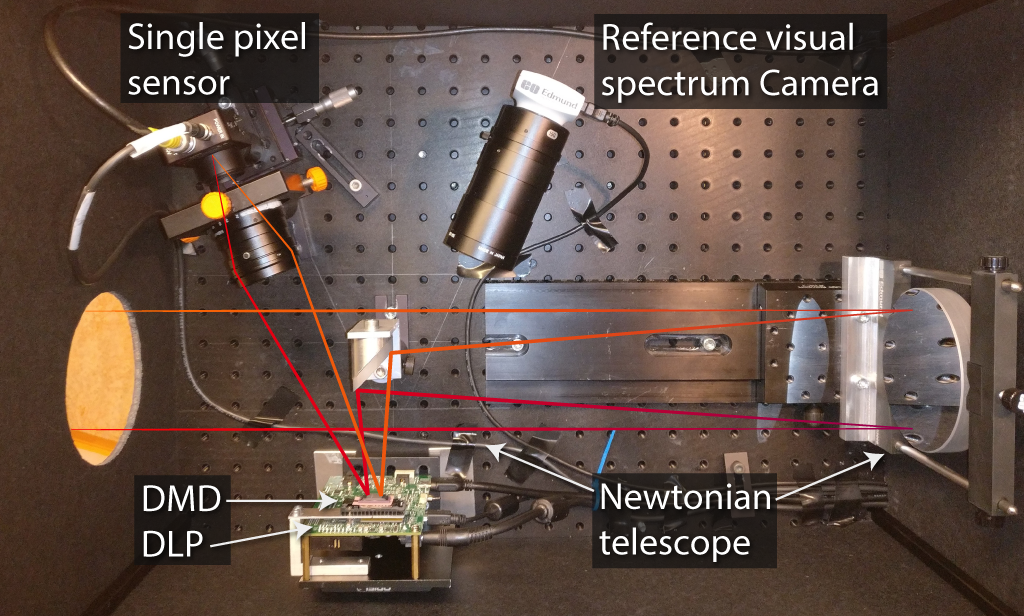
\includegraphics[width = 0.9\textwidth]{gfx/SPC.png}
    \caption{Single pixel imaging system (SPIS), adopted from \cite{article:foiSPIS}.}
    \label{fig:system1}
\end{figure}



As seen in figure~\ref{fig:system1} light from the scene is focused by the Newtonian telescope and reflected onto the DMD. The mirrors on the DMD can turned individually either into the single pixel sensor or the reference camera. The DMD acts as a Spatial Light Modulator (SLM) and reflects different patterns which is 'summed up' in the single pixel sensor as an intensity. The reconstructed image from the system will have the same resolution as the DMD patterns. The DLP is the DMD control unit which controls which patterns are displayed on the DMD either by reading images from memory or the video port.   


\subsubsection{Newtonian telescope}
A Newtonian telescope is a reflecting telescope, using a concave primary mirror and a flat diagonal secondary mirror, see figure~\ref{fig:system1}. In this set-up the telescope act as a lens focusing the scene onto the DMD. The motivation to use a Newtonian telescope instead of a lens system is partly that chromatic aberration is eliminated and partly that a reflective optical system works over a greater range of wavelengths that includes SWIR, near infrared (NIR) and the visible spectrum.

\subsubsection{DLP and DMD}
The DMD (Texas Instruments DLP4500NIR) is a matrix of micro mirrors that can be individually tilted $\pm 12^{\circ}$ and reflects wavelengths in the range 700-2500 nm. The DMD is controlled by the DLP (DLP LightCrafter 4500) which can be controlled either by video port (HDMI) or by the internal flash memory. The internal memory can theoretically be faster than the video port but due to constraints in both memory and memory bandwidth the fastest measurement matrix rate gets stuck at $270 - 300$ Hz. The video port can be operated at 120 Hz and display one bit plane at the time from a $24$ bit signal, which gives a maximum measurement matrix rate at $120 \times 24 = 2880$ Hz, but in the current configuration only $60$ Hz frame rate was achieved giving a measurement matrix rate at $1440$ Hz. At this rate with the number of measurements relative to number of pixels in reconstructed image between $20\% - 30\%$ a $256\times256$ pixel images data would be acquired in $9 - 13$ seconds and for a $512\times512$ pixel image $36-53$ seconds. To control the DMD the software 'DLP LightCrafter 4500 Control Software' is used.\\[0.1in] 

The DMD in the setup is constructed with a diamond shaped pattern instead of a regular square grid which is used in regular camera image sensors. The diamond shape causes the index of each mirror to be skewed against what a normal grid would look like. As seen in figure~\ref{fig:dmd_index} the indexes of the mirrors column is two mirror column arrays wide while a row is a single row. 


\begin{figure}[H]
    \centering
    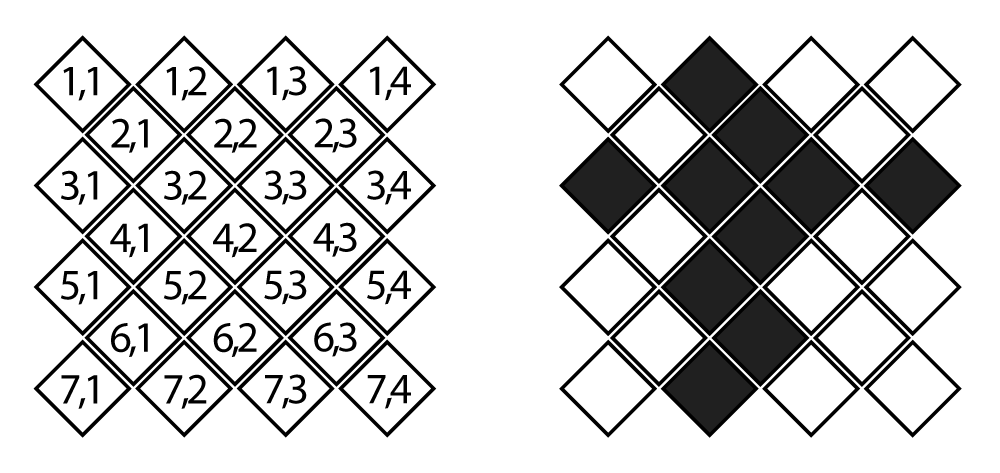
\includegraphics[width = 0.8\textwidth]{gfx/DMD_grid.png}
    \caption{DMD matrix, left shows each tiles index and right shows second row and second column in black.}
    \label{fig:dmd_index}
\end{figure}

Because the reconstruction algorithm and measurement matrix needs to be a square matrix with the side length with a power of 2 the resulting images ratio would be 2 to 1 while the image should have the ratio 1 to 1. The resulting image would need to be transformed into the real ratio where information potentially gets lost. Therefore the index of mirrors was changed so that each 'pixel' gets two mirrors as seen in figure~\ref{fig:dmd_index2}. This will result in rows and columns gets equal amount of space and the aspect ratio will be preserved to 1 to 1. 

\begin{figure}[H]
    \centering
    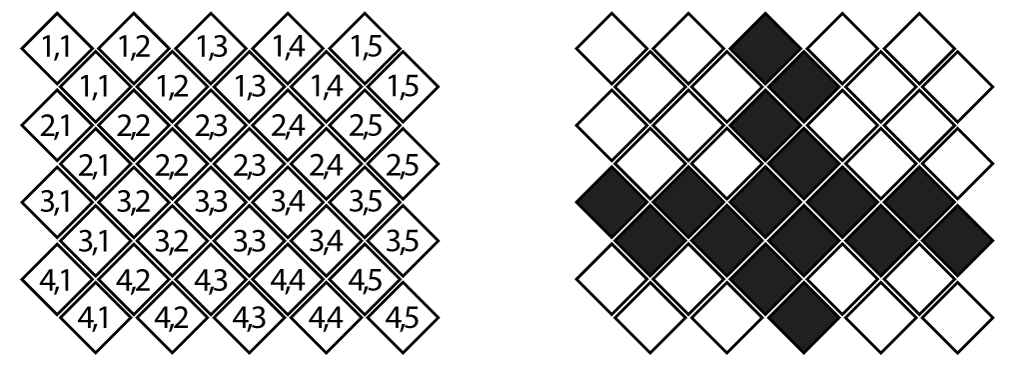
\includegraphics[width = 0.8\textwidth]{gfx/DMD_grid2.png}
    \caption{DMD matrix, left shows each tiles index and right shows third row and third column in black.}
    \label{fig:dmd_index2}
\end{figure}

\todo[inline]{Connect the DMD to CS and the physical aspect (every mirror is an pixel)} 


\begin{figure}[H]
    \centering
    
\includegraphics[width = 0.5\textwidth]{gfx/DMD_pattern.png}
    \caption{A typical measurement matrix presented on the DMD with the resolution $256 \times 256$ pixels.}
    \label{fig:dmd_pattern}
\end{figure}



\subsubsection{Lens}
The lens mounted on the single pixel sensor is an 50mm SWIR Fixed Focal Length Lens with an variable appature from f1.4 designed for wavelengths raging from the 800 nm in the visual spectrum to 2000 nm in the SWIR spectrum. \cite{website:SWIR_objective}

\subsubsection{Single pixel sensor}
The single pixel sensor is a Thorlabs PDA20C/M and is sensitive in wavelength range 800-1700 nm which is beyond the visual spectrum (390-700 nm). The sensor outputs an analog signal in volt which the sampler converts to a discret value. \cite{manual:PDA}

\subsubsection{Signal spectrum}
All components characteristics assembled the wavelengths that pass trough the system and measured in the single pixel sensor is between 800-1700 nm.



\subsection{Compressive imaging}
\todo[inline]{Write introduction to CS, create some intuition}
The single pixel sensor captures a scene by measuring the light intensity focused into the detector reflected from the DMD matrix. The DMD sensing matrix changes to obtain new measurements, $M$ unique sensing matrix measurements is captured to reconstruct an image with $N$ pixels. Each sensing matrix index is encoded either  by a one or a zero (turning the mirror onto or away from the sensor). The compressive imaging sampling model is defined as

\begin{equation}
\label{eq:CS1}
   \mathbf{ y = \Phi x + \epsilon}\text{,}
\end{equation}\\[0.1in]

where, $\mathbf{x}_{N\times1}$ is the signal (image) with $N$ samples (pixels), $\mathbf{y}_{M\times1}$ is the vector with $M$ measurements, $\mathbf{\Phi}_{M \times N}$ is the measurements matrix (each unique sensing matrix $\Phi_{1 \times N}$ as a row vector) and $\mathbf{\epsilon}$ is the noise. In conventional sampling the number of measurements $M$ needs to be at least equal to the number of samples $N$ to recover the signal but CS states that $M$ can be relatively small compared to $N$ given how compressible the signal is. The signal $\mathbf{x}$ can be represented as  

\begin{equation}
\label{eq:CS2}
   \mathbf{ \Psi \Theta = x }\text{,}
\end{equation}\\[0.1in]

where, $\mathbf{\Psi}_{N \times N}$ is some  basis matrix and
$\mathbf{\Theta}_{N\times1}$ is the coefficients where $\mathbf{\theta}$ is $K$-sparse. $K$-sparse means that the signal $\mathbf{x}$ has $K$ non zero elements in basis $\mathbf{\Psi}$, $||\mathbf{\Theta}||_0 = K$. Given equation~\ref{eq:CS2}, equation~\ref{eq:CS1} can be expand to


\begin{equation}
   \mathbf{ y = \Phi x + \epsilon = \Phi \Psi \Theta + \epsilon = A \Theta + \epsilon }\text{,}
\end{equation}\\[0.1in]

where, $\textbf{A}_{M \times N} = \Phi \Psi$ is the reconstruction matrix. The last statement is what makes CS powerful, a signal which is not sparse can be sampled with measurement matrix $\Phi$ and then reconstructed with reconstruction matrix $\textbf{A}$ in a basis where $\textbf{x}$ is sparse or compressible.
\subsection{Measurement matrix \& Restricted isometry property (RIP)}
\todo[inline]{Introduce the topic.}

In the noiseless case exact recovery of the image $\mathbf{x}$ is achievable if RIP holds for the reconstruction matrix $\mathbf{\Phi} \Rightarrow \mathbf{\Phi\Psi = A}$, the constraint is defined as,

\begin{equation}
    (1-\delta_K)||\mathbf{x}||_{\ell_2}^2\leq||\mathbf{Ax}||_{\ell_2}^2\leq(1+\delta_K)||\mathbf{x}||_{\ell_2}^2 \text{,}
\end{equation}\\[0.1in]

where $\delta_K \in [0.1)$ is the smallest constant to to satisfy RIP for a K-sparse signal $\mathbf{x}$. To determine a sampling matrix is a NP-hard problem (which means that there are no feasible way of creating a optimal reconstruction matrix) and generally $\textbf{x}$ is not known and varies which means that there are no general optimal reconstruction matrices for natural images. The solution is to find a general reconstruction matrix that satisfies RIP with high probability. The solution which also should be incoherent with the base matrix $\Psi$ is to construct the measurement matrix using a i.i.d random distribution which gives $\delta_K << 1$ with high probability. Using random measurement matrices the number of measurements needed to satisfy RIP with high probability is $M \geq O(K\text{log}(N/K) \ll N$.\\[0.1in]

The problem using random matrices is that they need to be stored i memory for the reconstruction algorithm, when the image resolution is increased the measurement matrix increases exponentially. For images with resolution of $512\times 512$ and larger the data gets infeasible for a normal computer to handle.  Fortunately using fast transforms in the reconstruction algorithm can exclude using vector multiplication resulting in faster reconstruction and the need to store the measurement matrix in memory. But in order to do so special measurement matrices are used, in this master's thesis the sequency ordered Walsh Hadamard measurement matrix will be used with the TVAL3 reconstruction algorithm described in section~\ref{sec:TV}.   


\subsubsection{Sequency ordered Walsh Hadamard measurement matrix}
Besides from eliminating the need to store the measuring matrix for reconstruction the sequency ordered Walsh Hadamard (SOWH) matrix can be generated when sent to the DMD eliminating the need to store the matrix at all. SOWH has the same characteristics and properties of an i.i.d random matrix and therefore also fulfills the RIP condition with high probability and research has shown that there is no significant loss in recovery of the signal relative i.i.d random measurement matrix. \todo{find the source ref} An other property of SOHW is that it only contains -1 an 1 which easily be converted to 0 and 1 when sent to the DMD. \\[0.1in]


The naturally ordered Hadamard matrix of dimension $2^k$, $k \in \mathbb{N}$ are constructed by the recursive formula    

\begin{equation}
    H_0 = 1,
\end{equation}

\begin{equation}
    H_1 = \begin{bmatrix}
       1 & 1 \\
       1 & -1\\
     \end{bmatrix},
\end{equation}

and in general,

\begin{equation}
        H_k = \begin{bmatrix}
       H_{k-1} & H_{k-1} \\
       H_{k-1} & -H_{k-1}\\
       \end{bmatrix} = H_1 \oplus H_{k-1}
\end{equation}

where $\oplus$ denotes the Kronecker product. To construct the sequency ordered Walsh Hadamard matrix from the naturally ordered Hadamard matrix three steps is required:

\begin{itemize}
    \item Convert row index to binary.
    \item Convert the binary row index to gray code.
    \item Apply bit reverse on the gray code index.
\end{itemize}

then order the rows after the bit reverse to obtain the sequency ordered Walsh Hadamard matrix.

\begin{table}[H]
\begin{tabular}{|r|c|c|c|c|}
\hline
    $n_H$        & 0    & 1     & 2     & 3     \\ \hline
    Binary       & 00   & 01    & 10    & 11    \\ \hline
    Gray code    & 00   & 01    & 11    & 10    \\ \hline
    Bit-reverse  & 00   & 10    & 11    & 01    \\ \hline
    $n_W$        & 0    & 2     & 3     & 1     \\ \hline
    
\end{tabular}
\label{tab:Hadamard_2_Walsh}
\caption{How to convert a naturally ordered Hadamard matrix to a sequency ordered Walsh Hadamard matrix by shifting row with index $n_W$ to $n_H$}
\end{table}

for example

\begin{equation}
    H_2 =  \begin{bmatrix}
       1 & 1 & 1 & 1 \\
       1 & -1 & 1 & -1 \\
       1 & 1 & -1 & -1 \\
       1 & -1 & -1 & 1 
       \end{bmatrix} \Rightarrow W_2 = \begin{bmatrix}
       1 & 1 & 1 & 1 \\
       1 & 1 & -1 & -1  \\
       1 & -1 & -1 & 1  \\
       1 & -1 & 1 & -1 
       \end{bmatrix}.
\end{equation}

To use the sequency ordered Walsh Hadamard matrix as an measurement matrix the fist row is omitted, permutations to the columns is performed, $M$ rows are choosen at random and the indices with a $-1$ is shifted to $0$. This last step is required to convert the measurement matrix so it gets the characteristics of an i.i.d random matrix and thus fulfill the RIP condition. How the matrix was permutated is stored because the reconstruction algorithm uses that information. \cite{article:WalshHadamard_Max_Length, article:TVAL3}. 

\subsection{Reconstruction method}
To reconstruct the image $\textbf{x}$ the sparest set of coefficients in $\Theta$ is desired. The optimal approach to find these coefficients would be to use $\ell_0$ minimization


\begin{equation}
   \mathbf{ \hat{\theta}} = \text{arg min } ||\mathbf{\theta}||_0 \text{  subject to  } \mathbf{y = A\theta} \text{.}
\end{equation}\\[0.1in]


Simply minimizing nonzero indices $\mathbf{\Theta}$ in the sparsitfying basis $\mathbf{\Psi}$, but this problem is known to be NP-hard. A better approach is the $\ell_1$ minimization, for example Basis Pursuit denoise (BPDN),

\begin{equation}
    \mathbf{\hat{\theta}} = \text{arg min } ||\mathbf{\theta}||_1 \text{  subject to  } ||\mathbf{y - A\theta}||_2 < \mathbf{\epsilon} \text{.}
\end{equation}\\[0.1in]

In 2006 Donoho~\cite{article:CS_donoho1} for the fist time guarantied theoretical $\ell_0\text{/}\ell_1$ equivalence which holds in the CS case, which means using a $\ell_1$ minimizer is guaranteed to find the sparsest solution in polynomial time in the noiseless case which can be approximated in the noisy and compressible signal case. The drawback with the $\ell_1$ minimizer is that it require more measurements than the optimal case with $\ell_0$ but it is still $M \ll N$. Since 2006 many more types of optimization algorithms has evolved which solves the problem with different methods but with the same goal: finding the largest most significant coefficients of $\mathbf{\theta}$. \todo{Why use the TV algorithm} 


\subsubsection{Total variation}
\label{sec:TV}
\todo[inline]{A closer look at the TVAL3 algorithm}
The reconstruction algorithm that was chosen in this Master's thesis was a total variation regularization algorithm. Natural images often contains sharp edges and piecewise smooth areas  which the TV regularization algorithm is good at preserving. 

TV
AL  Augmented Lagrangian - \todo[inline]{Augmented Lagrangian methods are a certain class of algorithms for solving constrained optimization problems. They have similarities to penalty methods in that they replace a constrained optimization problem by a series of unconstrained problems and add a penalty term to the objective; the difference is that the augmented Lagrangian method adds yet another term, designed to mimic a Lagrange multiplier.}
AL  Alternating Direction - \todo[inline]{Alternating direction methods are a common tool for general mathematical programming and
optimization. These methods have become particularly important in the field of variational image processing,
which frequently requires the minimization of non-differentiable objectives. This paper considers accelerated
(i.e., fast) variants of two common alternating direction methods: the Alternating Direction Method of
Multipliers (ADMM) and the Alternating Minimization Algorithm (AMA). The proposed acceleration is of
the form first proposed by Nesterov for gradient descent methods. In the case that the objective function is
strongly convex, global convergence bounds are provided for both classical and accelerated variants of the
methods. Numerical examples are presented to demonstrate the superior performance of the fast methods
for a wide variety of problems.}
\todo[inline]{The alternating direction method of multipliers (ADMM) is an algorithm that solves convex optimization problems by breaking them into smaller pieces, each of which are then easier to handle. It has recently found wide application in a number of areas. On this page, we provide a few links to to interesting applications and implementations of the method, along with a few primary references.

ADMM is used in a large number of papers at this point, so it is impossible to be comprehensive here. We only intend to highlight a few representative examples in different areas. To keep the listing light, we have only listed more detailed bibliographic information for papers that are not easy to find online; in any case, the information given should be more than enough to track down the papers.}
AL  Algorithm

\subsection{Image capturing and processing chain}
\todo[inline]{A section describing the process from sampling the signal to complete image. Which algorithms was used and an introduction to how the signal looks at different stages of the process.}
\todo[inline]{Flowchart of the whole process.}
\begin{itemize}
\item A video containing the measurement matrix with 24 matrices per frame was streamed was stream through a HDMI port with the software MPC-HC. The DLP shows one bit plane at the time on the DMD until next frame arrives. 
\item MATLAB was used for signal processing.
\item Acquire signal: Start sampling signal from the single pixel sensor, and start chain of measurement matrices.
\item From the raw signal: Extract value from each measurement matrix, Signal processing compensating for illumination change and delete if necessary disruption. We use the knowledge that the signal should be stationary.
\item Reconstruct image from signal.
\item Image processing: median filter. 
\end{itemize}

\pagebreak
\subsection{Evaluation: Image quality assessment}
The evaluation will be divided in to two categories: reconstructed images from synthetic data and images reconstructed from data acquired by the SPC.\\[0.1in] 

The evaluation on synthetic data is focused on evaluating the performance of the measurement matrix and reconstruction algorithm. Evaluating synthetic data gives two possibilities that can not be achieved with images reconstructed using the SPC which is that there is a reference image which the resulting image can be compared to.

Reconstructed image from synthetic data is acquired by creating a signal $ \mathbf{ y }_{M\times1}$ taking the inner product of $ \mathbf{y} = \mathbf{\Phi} \mathbf{x} + \epsilon$ where, $\mathbf{x}$ is the synthetic image reshaped to a vector, $\mathbf{\Phi}$ is the measurement matrix with the desired amount of measurements $M$ and synthetic noise $\epsilon$ which can be regulated to simulate different conditions, then using the reconstruction algorithm on the signal $\mathbf{y}$ to obtain the reconstructed image $\mathbf{\hat x}$. Because the measurement matrix and reconstruction algorithm is independent of the SPC hardware the subsystem can be evaluated independently. Two advantages of evaluation the sensing and reconstruction independently of the SPC is that parameters such as number of measurements and noise can be regulated easy and the second advantage is that a reference image is available for comparison.\\[0.1in] 

With a reference image available two image quality assessments are performed on the result from the simulation: Peak signal-to-nise ratio (PSNR) and  SSIM. PSNR is defined as

\begin{equation}
    \text{PSNR}[f(x,y),g(x,y)] = 10 log_{10}\frac{E^2}{\text{MSE}[f(x,y),g(x,y)]}
\end{equation}
 
where, $f(x,y)$ and $g(x,y)$ is intensity in pixel $(x,y)$...
 






\subsection{Method criticism}
\begin{itemize}
    \item No Reference Image Quality Assessment is not designed for SWIR images or SPC:s characteristics noise therefore the results may not reflect how the QA would answer to visual wavelength cameras. 
\end{itemize}
%LSE - absolute error but does not say much about how humans perceives the image.\\


\section{Evaluation}
\label{sec:Evaluation}
This section is structured as, for each experiment and setup a detailed explanation and motivation on how and why the experiment is needed followed by the results of that experiment. The experiments are motivated by gathering as much information and results as possible to answer the research questions. The first subsection~\ref{sec:simulated_results} will present the results from experiments with synthetic data where a reference image is available. The second subsection~\ref{sec:eval_spc} will present the result from images reconstructed from the SPC. No perfect reference image is available in those experiments therefore the images will be evaluated against near optimal image, no reference QA and against a state of the art SWIR camera. 



\subsection{Simulated results}
\label{sec:simulated_results}
In this section the results produces was simulated by using the reconstructing algorithm and measurement matrix described in section~\ref{sec:TV} and \ref{sec:SOWHMM} on high quality images captured with a state of the art SWIR camera. The images captured by the SWIR camera acts as a ideal reference to the reconstructed images. By simulating the result from "ideal" images the reconstruction process gets a benchmark independent of the SPC.


\subsubsection{Reconstruction performance using reference image}
\label{sec:reconstruction_performance}
In these simulation XX images captured by a state of the art SWIR camera was reconstructed, the performance of the reconstruction was calculated using PSNR and SSIM. Different degree of noise was added to the signal vector to simulate noise from the SPC where the largest added noise could not reconstruct the image at all. The test also simulates different under sampling ratios $\frac{M}{N}$ ranging from 5\% to 30\%. 

\todo[inline]{Add pictures of the simulated result}

\begin{figure}[H]
    \centering
    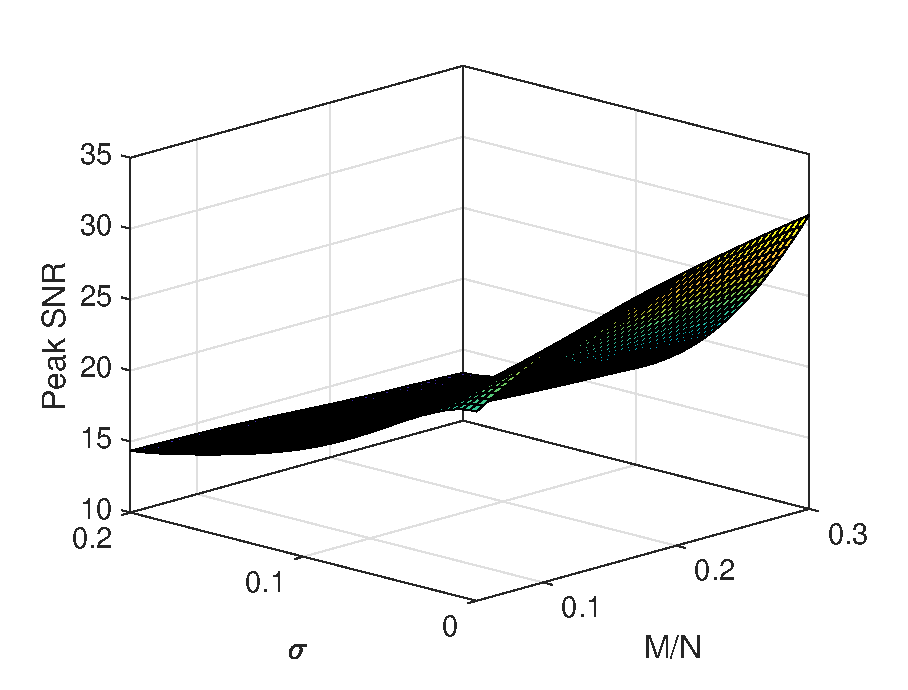
\includegraphics[width = 0.7\linewidth]{result/synt_sss/PSNR_fit.eps}
    \caption{Peak SNR result depending on number of measurements and simulated noise level.}
    \label{fig:psnr_3d}
\end{figure}
\todo[inline]{Change to dB}

\begin{figure}[H]
    \centering
    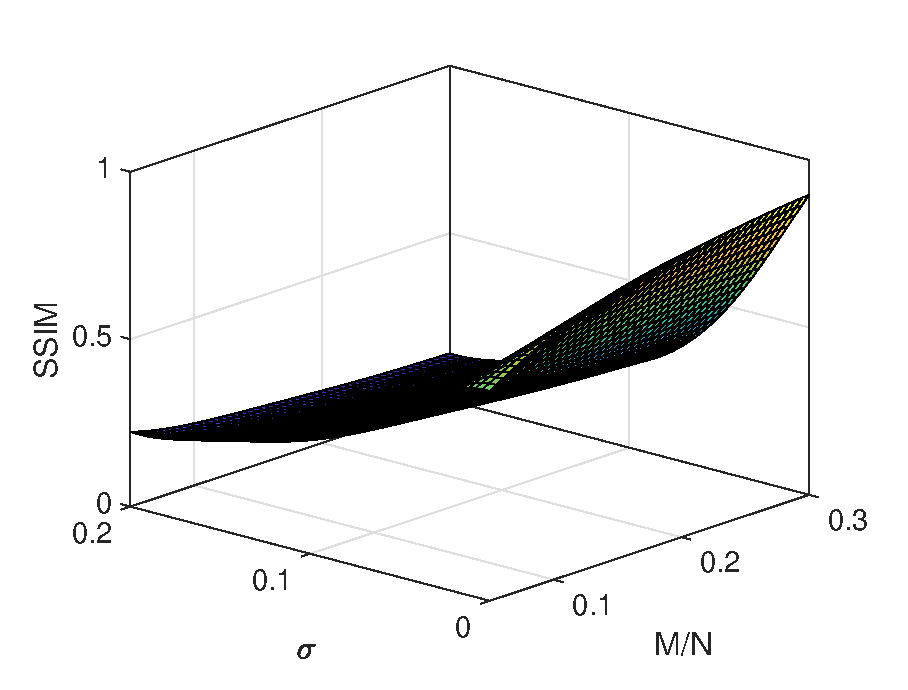
\includegraphics[width = 0.7\linewidth]{result/synt_sss/SSIM_fit.eps}
    \caption{SSIM result depending on number of measurements and simulated noise level.}
    \label{fig:ssim_3d}
\end{figure}

In figure~\ref{fig:psnr_3d} and \ref{fig:ssim_3d} the reconstruction performance is presented in PSNR and SSIM score respectively. The reconstitution performance is increased when the under sampling ratio is increased and when the noise is decreased.  

\subsubsection{Reconstruction performance using no reference quality assessment}
BRISQUE lower score is better.

\begin{figure}[H]
    \centering
    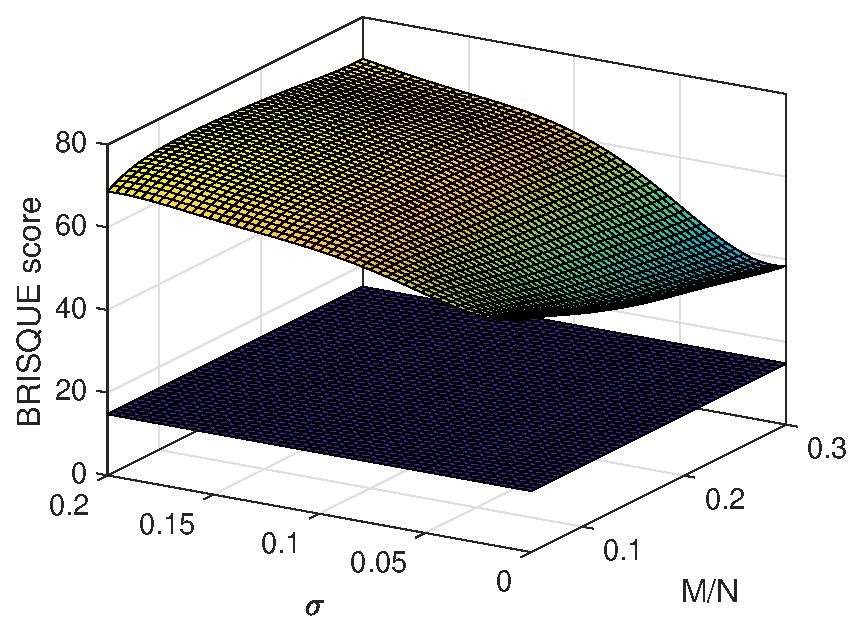
\includegraphics[width = 0.7\linewidth]{result/synt_brisque/BRISQUE_fit.eps}
    \caption{BRISQUE result depending on number of measurements and simulated noise level. Lower surface is reference image score.}
    \label{fig:Brisque_3d}
\end{figure}

\begin{figure}[H]
    \centering
    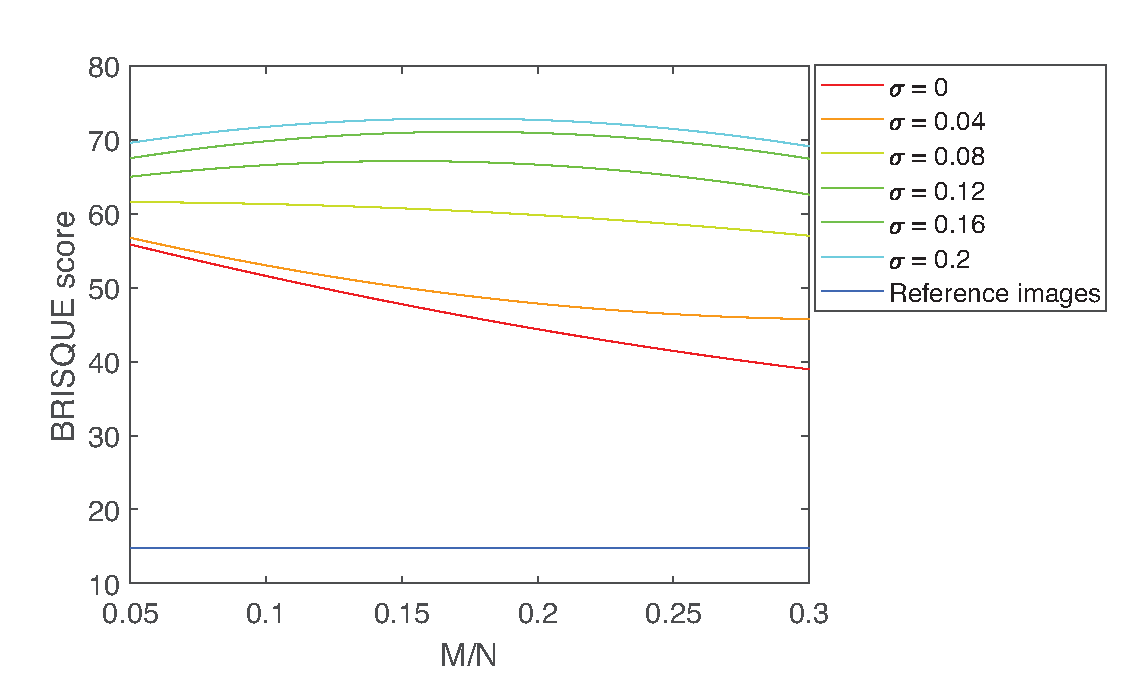
\includegraphics[width = 0.95\linewidth]{result/synt_brisque/Brisque_fit_flat3.eps}
    \caption{BRISQUE result depending on number of measurements for different simulated noise levels.}
    \label{fig:Brisque_2d}
\end{figure}
\todo[inline]{Add "optimal performance into the graph"}








\subsubsection{Dynamics in scene}
\label{sec:dyn_sim}
In the SPC setup, the exposure time was between 10 to 50 seconds, which increased the risk of dynamics in the scene. Dynamics in the scene reduces the reconstruction performance because the scene is assumed to be constant. By simulating dynamic scenes in a controlled environment, their individual effects to the sampled signal $\mathbf{y}$ could be identified and evaluated. As mentioned in section~\ref{sec:Dynamics_in_scene} dynamics in the scene can roughly be divided into two separate categories, luminance change and movement. In this section, global luminance change and two kinds of movement are simulated. The goal was to see how the signal changes when dynamics are introduced in the scene. In the case of luminance change, the moving mean algorithm presented in section~\ref{sec:Dynamics_in_scene} was evaluated.\\[0.1in]

To generate a simulated measurement representing a dynamic scene each sample $\mathbf{y}[m]$ is constructed using a unique image $\mathbf{x}_m$, which has been changed from the previous image,

\begin{equation}
\mathbf{y}[m] = \mathbf{\phi}_m\mathbf{x}_m.
\end{equation}

In the first scenario an object was placed in an image, but for each measurement the location of the object was be moved in a small bounded area of the image. Consequently, his model represents a scene where the background is static with a person moving in a small area.



\begin{figure}[H]
    \centering
\advance\leftskip-2cm
\begin{minipage}[t]{0.65\textwidth}
    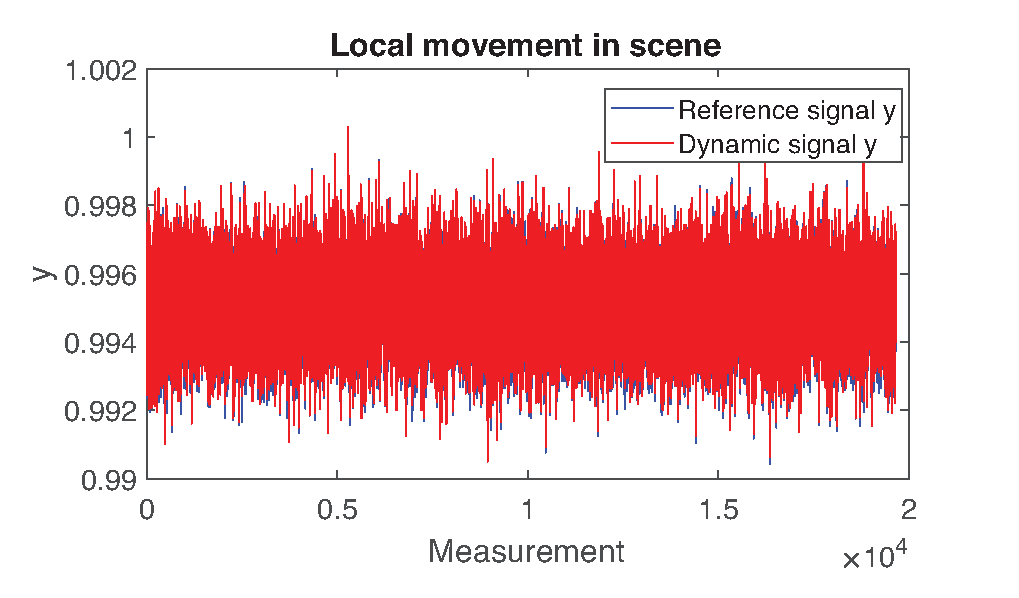
\includegraphics[width=1\textwidth]{result/dynamic/local/local_whole_time1.eps}
    \subcaption{}
    \label{fig:local_sig_1}
\end{minipage}
\advance\rightskip-2.0cm
\begin{minipage}[t]{0.55\textwidth}
    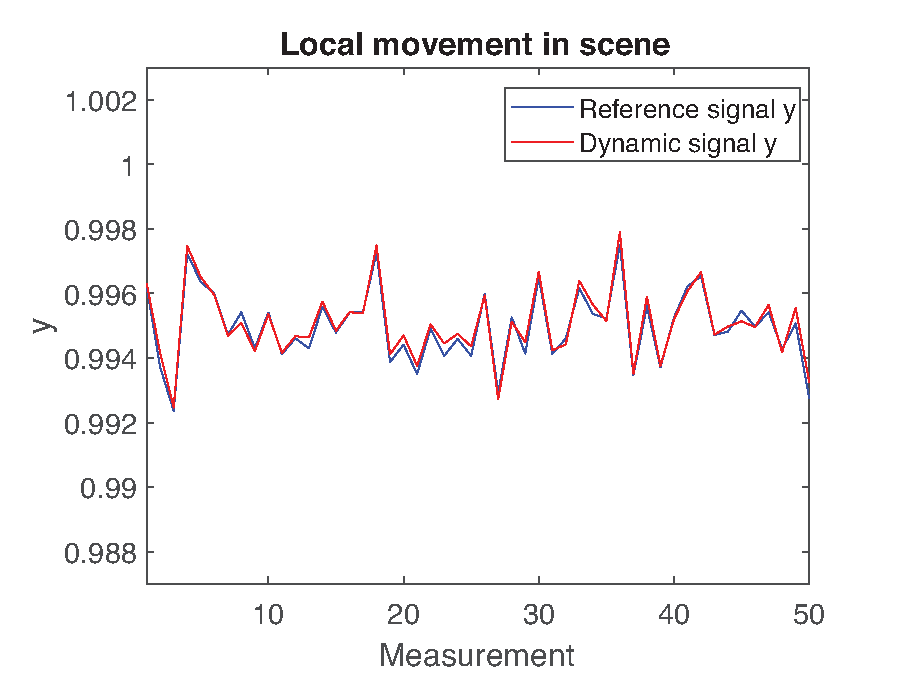
\includegraphics[width = \textwidth]{result/dynamic/local/local_whole_time_win1.eps}
    \subcaption{}
    \label{fig:local_sig_2}
\end{minipage}
    \caption{(a) Pertubated signal from local movement on top of reference signal. (b) Zoomed in view of some samples from figure (a).}
    \label{fig:local_sig}
\end{figure}

As seen in figure~\ref{fig:local_sig_1} there was no obvious difference between the non perturbed reference signal and the distorted signal. Neither in the zoomed in view in figure~\ref{fig:local_sig_2}, any large difference can be seen.\\[0.1in]

The reconstructed images from the reference signal and the perturbed signal are displayed in figure~\ref{fig:local_2} and \ref{fig:local_3}, respectively. The difference between the images are visible to the naked eye. Not only does the moving object get blurry and noisy, but the whole image globally.


\begin{figure}[H]
    \centering
\begin{minipage}[t]{0.32\textwidth}
    
\includegraphics[width=1\textwidth]{result/dynamic/local/local_whole_time_org.png}
    \subcaption{}
    \label{fig:local_1}
\end{minipage}
\begin{minipage}[t]{0.32\textwidth}
    
\includegraphics[width = \textwidth]{result/dynamic/local/local_whole_time_ref.png}
    \subcaption{}
    \label{fig:local_2}
\end{minipage}
\begin{minipage}[t]{0.32\textwidth}
    
\includegraphics[width = \textwidth]{result/dynamic/local/local_whole_time_res_psnr_29_snr_25_sssim_91.png}
    \subcaption{}
    \label{fig:local_3}
\end{minipage}
    \caption{The results of local movement in a reconstructed image, subsampled at 30\%. (a) Original reference image. (b) Reference image reconstructed from the original image without movement. (c) Reconstructed image from a scene with local movement.}
    \label{fig:local_dyn}
\end{figure}

In table~\ref{tab:local_dyn} the results from calculating PSNR and SSIM of the the reconstructed images are presented. It can be observed that the dynamic test image has been affected to some degree by the movement.

\begin{table}[H]
    \centering
  \begin{tabular}{ | l | l |}
    \hline
    Peak SNR  & SSIM \\ \hline
    29  & 0.91 \\ 
    \hline
  \end{tabular}
      \caption{Evaluation comparing a unperturbed reconstructed images against reconstructed images with local movement.}
    \label{tab:local_dyn}
\end{table}


%The conclusion of this test implies that local movement in a scene will cause noise in the image globally and especially locally where the movement occurred. It also implies that local movement is very hard to detect in the signal even if a reference signal is available.\\[0.1in]



%%%%%%%%%% Second scenario %%%%%%%%%%%%%%%%

The second scenario is an object passing through the whole scene. The problem is modeled with a static background and a simulated object crossing the whole scene, like a car, human or animal might do when using the SPC. The object will cross the scene in 1000 measurements of approximately 19000 in total which corresponds to approximately $0.7$ seconds, when sampling with the SPC in its current setup.\\[0.1in]



\begin{figure}[H]
    \centering
\begin{minipage}[t]{0.53\textwidth}
    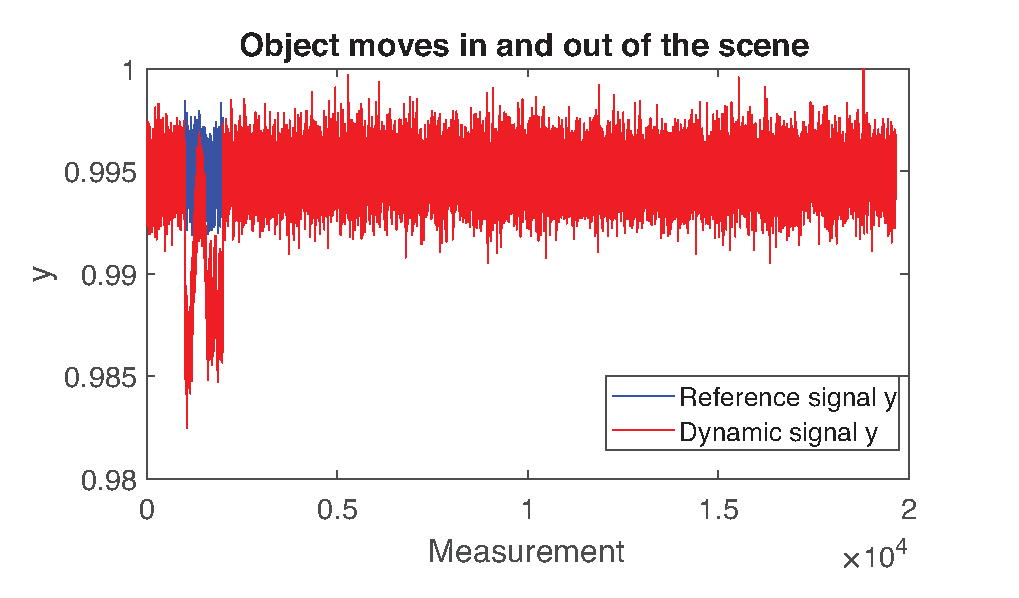
\includegraphics[width=1\textwidth]{result/dynamic/fly/flyby_sig1.eps}
    \subcaption{}
    \label{fig:fly_sig_1}
\end{minipage}
\begin{minipage}[t]{0.46\textwidth}
    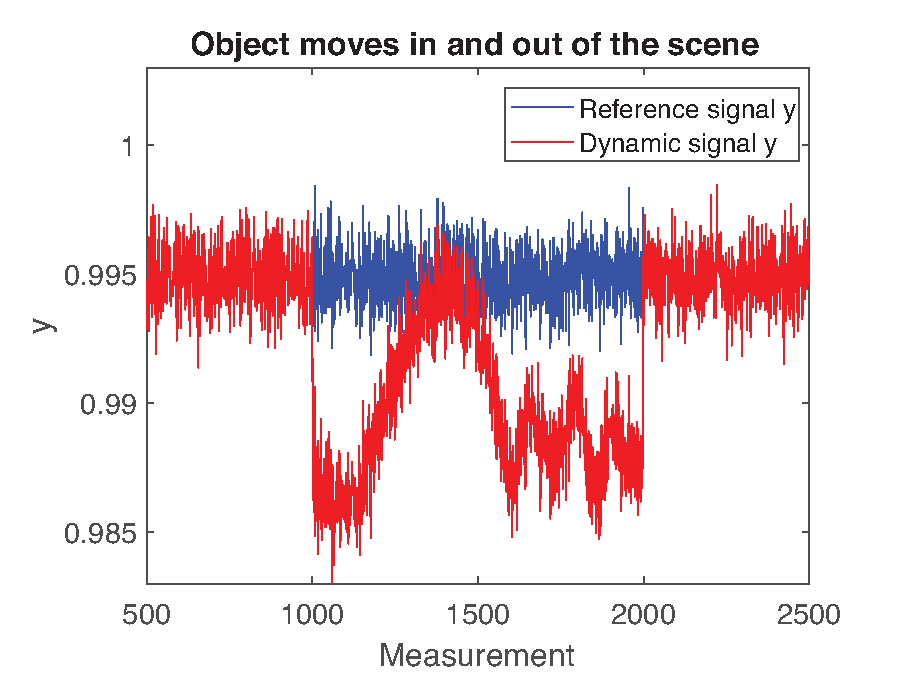
\includegraphics[width = \textwidth]{result/dynamic/fly/flyby_plot_win1.eps}
    \subcaption{}
    \label{fig:fly_sig_2}
\end{minipage}
    \caption{(a) Pertubated signal from large movement on top of the reference signal. (b) Zoomed in view of some samples from figure (a).}
    \label{fig:fly_sig}
\end{figure}

As seen in figure~\ref{fig:fly_sig}, at measurement 1000 the exact moment the object enters the scene, the signal changes. This is because a completely new structure has entered the scene and therefore the DC level changes. It can also be noted that after a while the object passed something which has approximately the same intensity as the background and therefore the DC signal almost returns to its original value for a brief moment.\\[0.1in] 

In figure~\ref{fig:fly_dyn} the effect of the moving object can be seen in the reconstructed image, which has gained a lot of global noise. Note that the object passing trough can not be seen because there is more measurements of the background than of the moving object. Nevertheless, the object is creating uncertainty in the whole image, resulting in global noise.   

\begin{figure}[H]
    \centering
\begin{minipage}[t]{0.32\textwidth}
    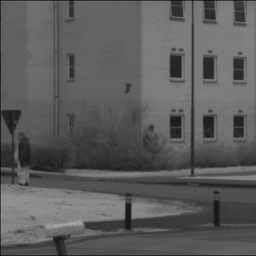
\includegraphics[width=1\textwidth]{result/dynamic/fly/flyby_1sec_org.png}
    \subcaption{}
    \label{fig:fly_1}
\end{minipage}
\begin{minipage}[t]{0.32\textwidth}
    
\includegraphics[width = \textwidth]{result/dynamic/fly/flyby_1sec_ref.png}
    \subcaption{}
    \label{fig:fly_2}
\end{minipage}
\begin{minipage}[t]{0.32\textwidth}
    
\includegraphics[width = \textwidth]{result/dynamic/fly/flyby_1sec_res_psnr_23_snr_18_sssim_58.png}
    \subcaption{}
    \label{fig:fly_3}
\end{minipage}
    \caption{The results of large movement on a reconstructed image, subsampled at 30\%. (a) Original reference image. (b) Reference image reconstructed from the original image without movement. (c) Reconstructed image from a scene with an object passing trough.}
    \label{fig:fly_dyn}
\end{figure}

In table~\ref{tab:fly_dyn} the results from calculating PSNR and SSIM of the reconstructed images are presented. It can be observed that the image has been effected heavily by the movement, lowering the SSIM index to 0.58. 


\begin{table}[H]
    \centering
  \begin{tabular}{ | l | l |}
    \hline
    Peak SNR  & SSIM \\ \hline
    23 &  0.58 \\ 
    \hline
  \end{tabular}
      \caption{Evaluation comparing unperturbed reconstructed image against reconstructed image with movement.}
    \label{tab:fly_dyn}
\end{table}


%Obviously in this context the samples with movement is very easy to spot and the easiest fix would be to just remove those measurements, reconstructing an image with fewer measurements. The resulting image would not be as good as the image in figure~\ref{fig:fly_2} but it would not be contain the noise present in figure~\ref{fig:fly_3}.\\[0.1in]



%%%%%%%%%%%% Third %%%%%%%%%%%%%%%

The third scenario is luminance change in the scene caused by inconsistency of light intensity from the source. Outdoors this means that the light intensity from the sun will vary over time, the most obvious being clouds occluding the sun but for example even change in air density can change the intensity. This scenario is modeled by adding or subtracting the global intensity in the image over the measurements. 

\begin{figure}[H]
    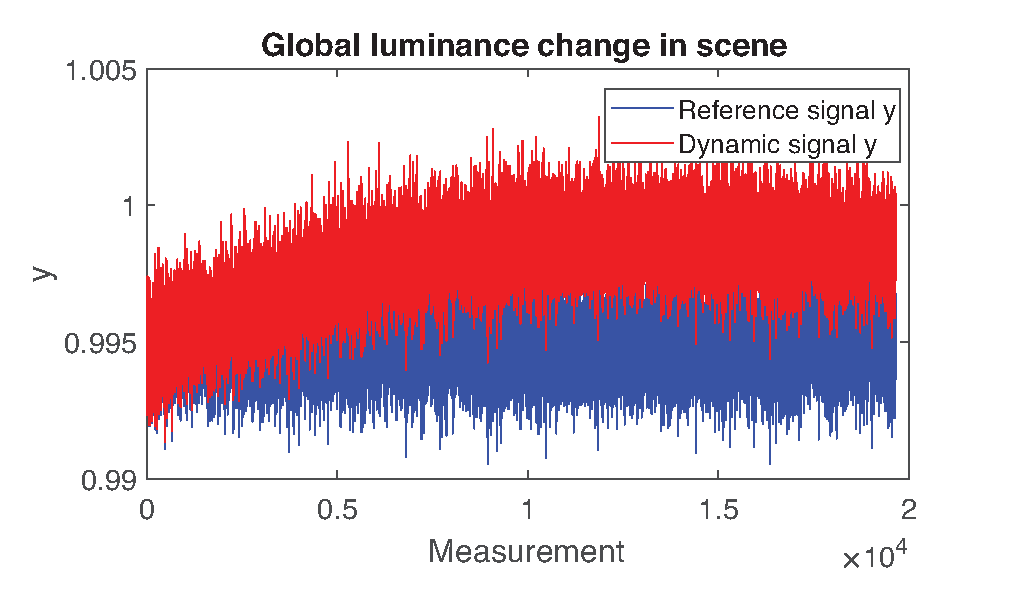
\includegraphics[width=0.6\textwidth]{result/dynamic/lum/intense_change1.eps}
    \caption{Signal effected by light intensity change on top of reference signal.}
    \label{fig:lum_sig_1}
\end{figure}

As seen in figure~\ref{fig:lum_sig_1}, the DC level of the signal will slowly change, but the structure of the signal stay the same. In figure~\ref{fig:lum_dyn} the reconstructed images from the perturbed signal and the reference signal are displayed. The reconstructed image from the dynamic signal has gained a lot of global noise even though the structure in the image has not been changed over the measurements.  


\begin{figure}[H]
    \centering
\begin{minipage}[t]{0.32\textwidth}
    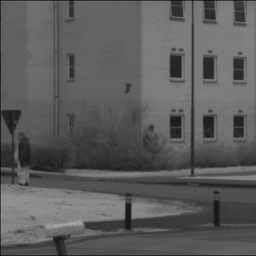
\includegraphics[width=1\textwidth]{result/dynamic/lum/intense_change_org.png}
    \subcaption{}
    \label{fig:lum_1}
\end{minipage}
\begin{minipage}[t]{0.32\textwidth}
    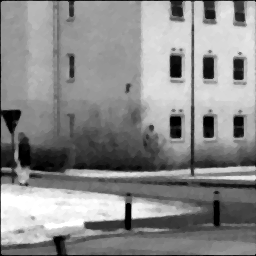
\includegraphics[width = \textwidth]{result/dynamic/lum/intense_change.png}
    \subcaption{}
    \label{fig:lum_2}
\end{minipage}
\begin{minipage}[t]{0.32\textwidth}
    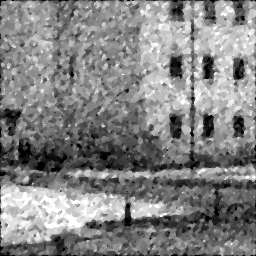
\includegraphics[width = \textwidth]{result/dynamic/lum/intense_change_psnr_19_snr_14_sssim_38.png}
    \subcaption{}
    \label{fig:lum_3}
\end{minipage}
    \caption{The result of global light intensity change on a reconstructed image subsampled at 30\% (a) Original reference image. (b) Reference image reconstructed from the original image without light intensity change. (c) Reconstructed image from a scene with global light intensity change over the measurements.}
    \label{fig:lum_dyn}
\end{figure}

In section~\ref{sec:Dynamics_in_scene}, a model of this problem was proposed along with an algorithm to suppress the impact of global luminance change. The algorithm is applied to this experiment to evaluate its performance. The moving mean subtraction method is applied and in figure~\ref{fig:lum_sig_2} the resulting signal is plotted over the dynamic signal. Note that the processed signal is stationary again. In figure~\ref{fig:lum_sig_3} and \ref{fig:lum_sig_4}, where the processed signal is plotted over the reference signal, it can be seen that the processed signal has gained its original structure and almost fit exactly to the original.


\begin{figure}[H]
    \centering
\begin{minipage}[t]{0.48\textwidth}
    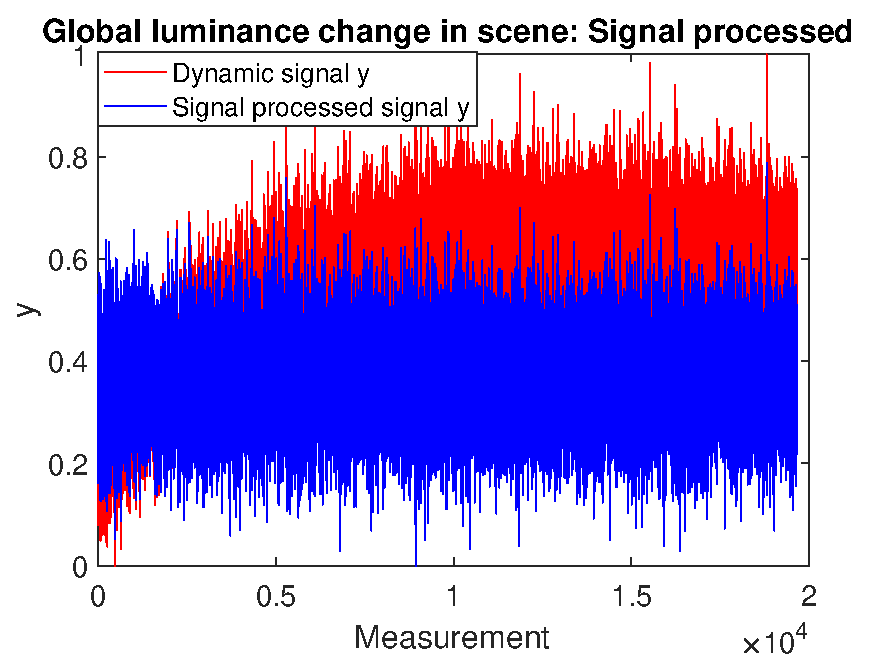
\includegraphics[width = \textwidth]{result/dynamic/lum/intense_change_sp.eps}
    \subcaption{}
    \label{fig:lum_sig_2}
\end{minipage}
\begin{minipage}[t]{0.51\textwidth}
    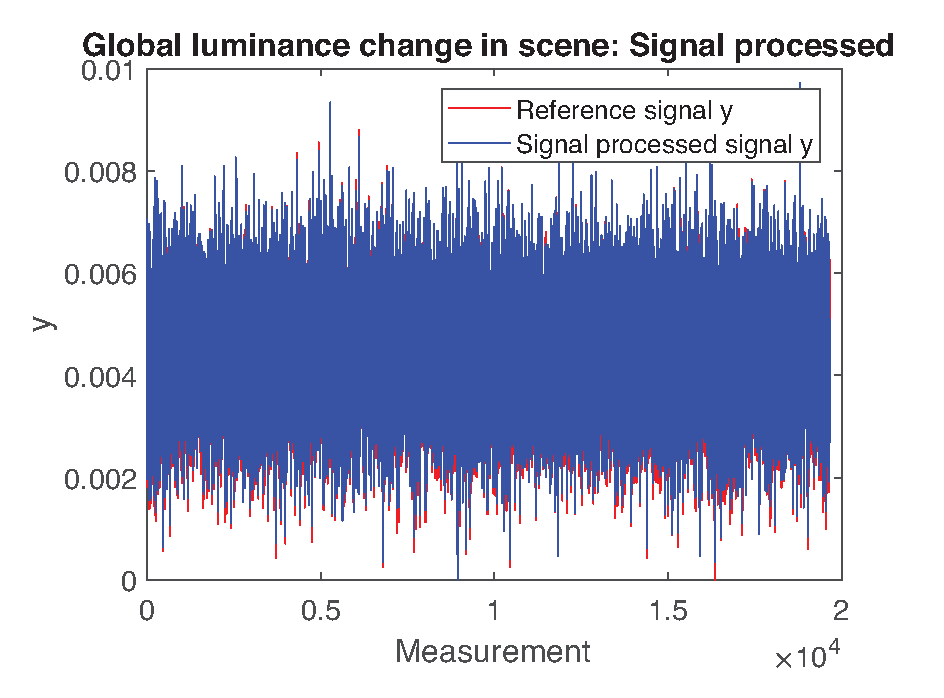
\includegraphics[width=1\textwidth]{result/dynamic/lum/intense_change_sp_ref1.eps}
    \subcaption{}
    \label{fig:lum_sig_3}
\end{minipage}
\begin{minipage}[t]{0.50\textwidth}
    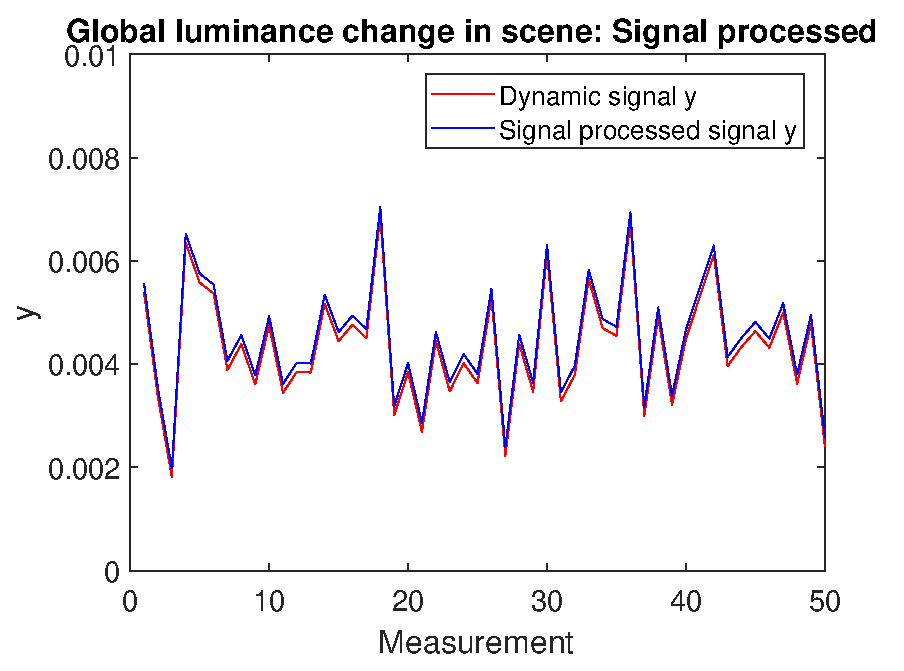
\includegraphics[width = \textwidth]{result/dynamic/lum/intense_change_sp_ref_win.eps}
    \subcaption{}
    \label{fig:lum_sig_4}
\end{minipage}
    \caption{Post-processed signal using moving mean subtraction. (a) Post-processed signal on top of the dynamic signal. (b) Post-processed signal on top of the reference signal. (c) Zoomed in view of (b).}
    \label{fig:lum_sig}
\end{figure}

In figure~\ref{fig:lum_rec}, the processed signals reconstructed image is displayed between the reference and perturbed signals reconstructed images. The moving mean algorithm improve the reconstruction significantly, the image has gained some noise compared to the reference image, but over all there is not much difference between them.


\begin{figure}[H]
    \centering
\begin{minipage}[t]{0.32\textwidth}
    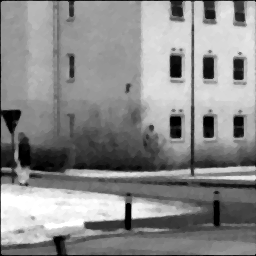
\includegraphics[width = \textwidth]{result/dynamic/lum/intense_change.png}
    \subcaption{}
    \label{fig:lum_22}
\end{minipage}
\begin{minipage}[t]{0.32\textwidth}
    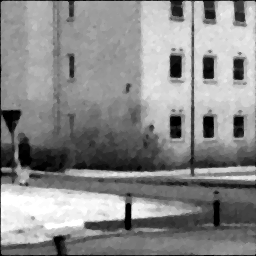
\includegraphics[width = \textwidth]{result/dynamic/lum/intense_change_movemean_psnr_33_snr_29_sssim_93.png}
    \subcaption{}
    \label{fig:lum_4}
\end{minipage}
\begin{minipage}[t]{0.32\textwidth}
    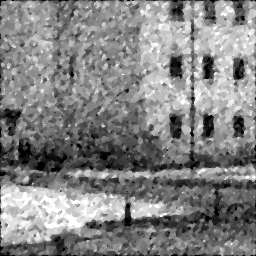
\includegraphics[width = \textwidth]{result/dynamic/lum/intense_change_psnr_19_snr_14_sssim_38.png}
    \subcaption{}
    \label{fig:lum_32}
\end{minipage}
    \caption{The result of processed signal perturbed by light intensity change on a reconstructed image subsampled at 30\% (a) Reference image reconstructed from the non perturbed signal without light intensity change. (b) Reconstructed image from a scene with global light intensity change and post processed by moving mean subtraction. (c) Reconstructed image from a scene with global light intensity change over the measurements.}
    \label{fig:lum_rec}
\end{figure}

In table~\ref{tab:lum_dyn} the results from calculating PSNR and SSIM of the reconstructed images are presented. Both PSNR and SSIM are increased for the reconstructed image using moving mean subtraction.


\begin{table}[H]
    \centering
  \begin{tabular}{ | l | l | l |}
    \hline
    Signal & Peak SNR  & SSIM \\ \hline
    Perturbed signal & 19  & 0.38 \\ \hline
    Mean subtracted signal & 33  & 0.93 \\
    \hline
  \end{tabular}
      \caption{Evaluation comparing unperturbed reconstructed image against global luminance change reconstructed image and moving mean subtracted signal processed reconstructed image.}
    \label{tab:lum_dyn}
\end{table}







\subsection{SPC evaluation}
\label{sec:eval_spc}
The evaluation section is now shifted to examine the images produced by the SPC. The images will be analyzed using the using a range of methods to examine the performance of the SPC. In this section the BRISQUE algorithm will be used again where connections to the previous result is drawn, a reconstructed image will be compared to an ideal image using homography, a set of images is presented reconstructed at different subsampling ratios, a edge response analysis i performed and the correlation between reconstruction performance and noise is conducted. 

\todo[inline]{The images captured was taken at a distance between 200 to 900 m}

\todo[inline]{List the specs?}

\subsubsection{Reconstructed performance Using reference image}
This evaluation is designed to get a measurement of expected image quality with the same metrics used in the synthetic case. As stated before, it is hard to obtain a reference image to the images produced by the SPC. One solution to obtain a reference image is to calculate a homography between images. But there are two problems of just performing a homography to obtain a reference image, the fist on is that, homography estimates the transformation between flat surfaces which excludes most natural images, and the second is that, the estimated homography will not be perfect an thus for example high contrast edges in the images will not match and then produce large errors in the performance measurements. To solve these two problems the scene is a flat surface with a printed pattern and to avoid the the error from sharp edges the pettern is constructed without any. To not complicate this experiment the reference image is the computer generated optimal images which is being transformed to fit the image captured by the SPC.\\[0.1in] 

The reference homography transformed image which was created using sine functions to avoid edges can be seen in figure~\ref{fig:hom_over_im} with the reconstructed images with different subsampling ratio.   


\begin{figure}[H]
    \centering
\begin{minipage}[h]{0.3\textwidth}
	\vspace*{1cm}
    
\includegraphics[width=1\textwidth]{result/hom/im_ref.png}
    \subcaption{Homography transformed refrence image}
    \label{fig:hom_ref}
\end{minipage}
\begin{minipage}[t]{0.22\textwidth}
    
\includegraphics[width = \textwidth]{result/hom/im_m5.png}
    \subcaption{5\%}
    \label{fig:hom_5}
    
\includegraphics[width = \textwidth]{result/hom/im_m20.png}
    \subcaption{20\%}
    \label{fig:hom_20}
\end{minipage}
\begin{minipage}[t]{0.22\textwidth}
    
\includegraphics[width = \textwidth]{result/hom/im_m10.png}
    \subcaption{10\%}
    \label{fig:hom_10}
    
\includegraphics[width = \textwidth]{result/hom/im_m25.png}
    \subcaption{25\%}
    \label{fig:hom_25}
\end{minipage}
\begin{minipage}[t]{0.22\textwidth}
    
\includegraphics[width = \textwidth]{result/hom/im_m15.png}
    \subcaption{15\%}
    \label{fig:hom_15}
    
\includegraphics[width = \textwidth]{result/hom/im_m30.png}
    \subcaption{30\%}
    \label{fig:hom_30}
\end{minipage}
    \caption{The reconstructed images with different number of measurements and the reference image transformed to fit the SPC images using homography.}
    \label{fig:hom_over_im}
\end{figure}

Before the results from the evaluation is presented it is worth noting that the reference image is a perfect simulated reference image, which was not effected by the uneven light source and quality of the print as the reconstructed image from the SPC, which for example can be seen in the edges of the reconstructed images in figure~\ref{fig:hom_5} to \ref{fig:hom_30}. In figure~\ref{fig:hom_score} below the same evaluation method as the reconstructed simulated images in section~\ref{sec:simulated_results} is used, PSNR and SSIM, because there is a reference image again. 


\begin{figure}[H]
    \centering
\begin{minipage}[t]{0.49\textwidth}
    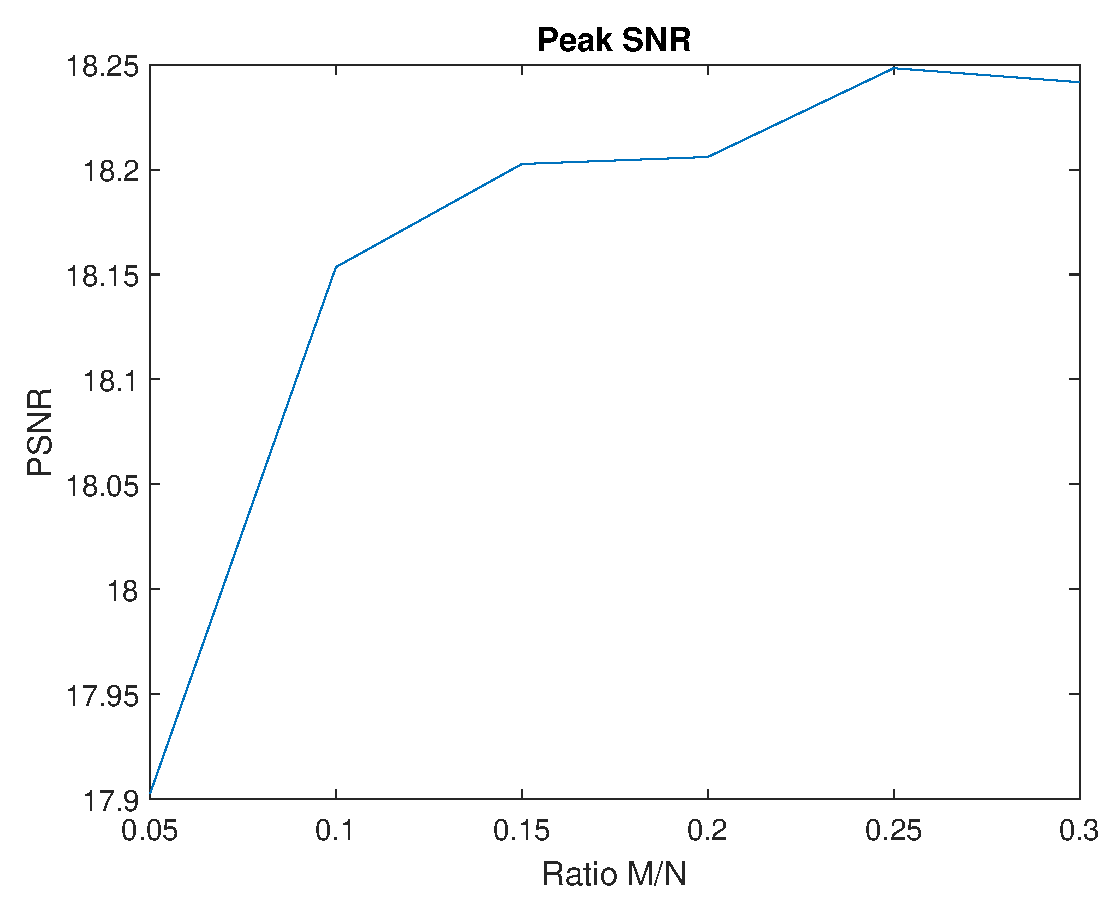
\includegraphics[width=1\textwidth]{result/homo/PSNR_2.eps}
    \subcaption{}
    \label{fig:hom_psnr}
\end{minipage}
\begin{minipage}[t]{0.49\textwidth}
    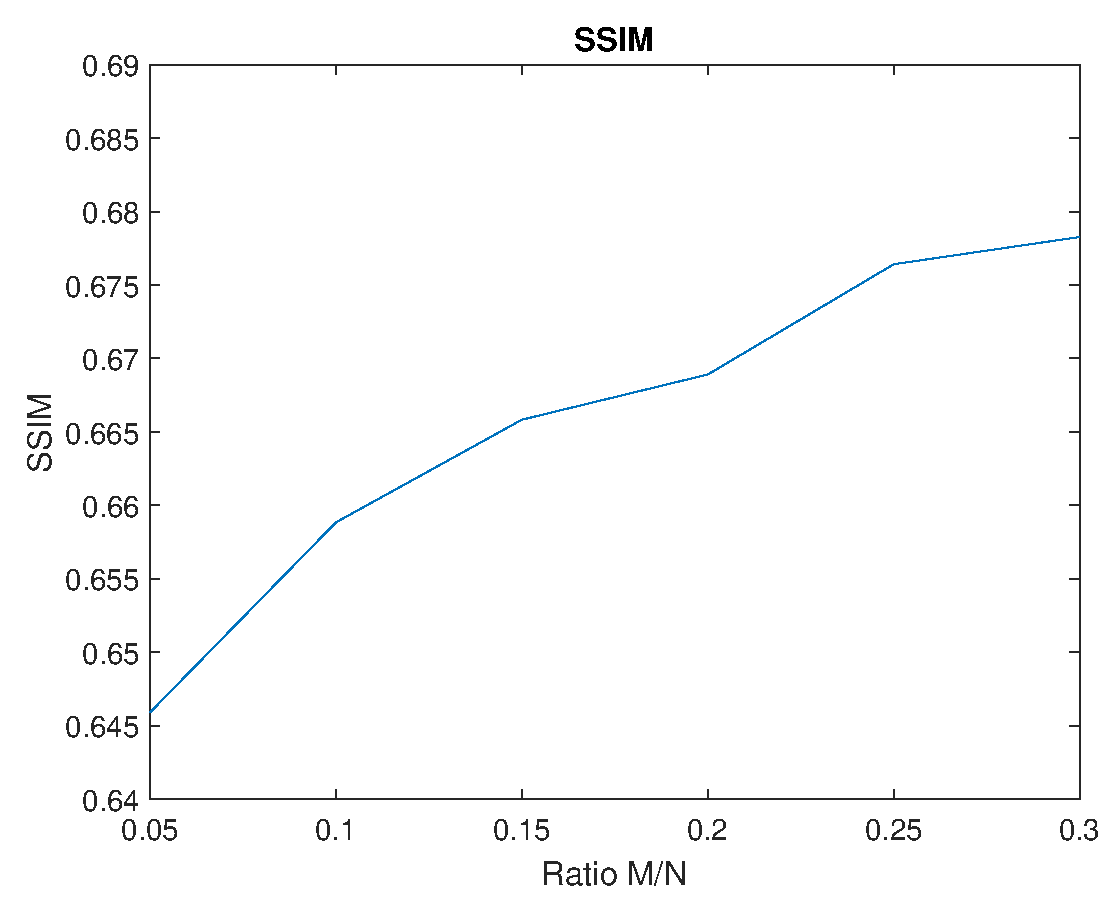
\includegraphics[width=1\textwidth]{result/homo/SSIM_2.eps}
    \subcaption{}
    \label{fig:hom_ssim}
\end{minipage}
    \caption{Signal quality of SPC images compared to reference image. (a) Peak SNR for reconstructed images against reference image. (b) SSIM score for reconstructed images against reference image.}
    \label{fig:hom_score}
\end{figure}

The result shows the same expected result as before with increased quality with increased subsample ratio. An second observation confirms the observation made in section~\ref{sec:measurements}, where the image quality is rapidly improves when increasing subsample ratio to to 15\%, then the improvement rate stagnates. 



\subsubsection{Reconstruction performance Using no reference quality assessment}
\label{sec:SPC_BRISQUE}
In this section the blind quality assessment tool BRISQUE will be used to score the reconstructed images from the SPC. The same algorithm was used on the simulated data where a benchmark was set as a theoretical limit to the reconstructed images.\\[0.1in]     

Each image is evaluated at subsampling rate from $5\%$ to $30\%$ where the result is presented in figure~\ref{fig:brisque_plot}.

\begin{figure}[H]
    \centering
    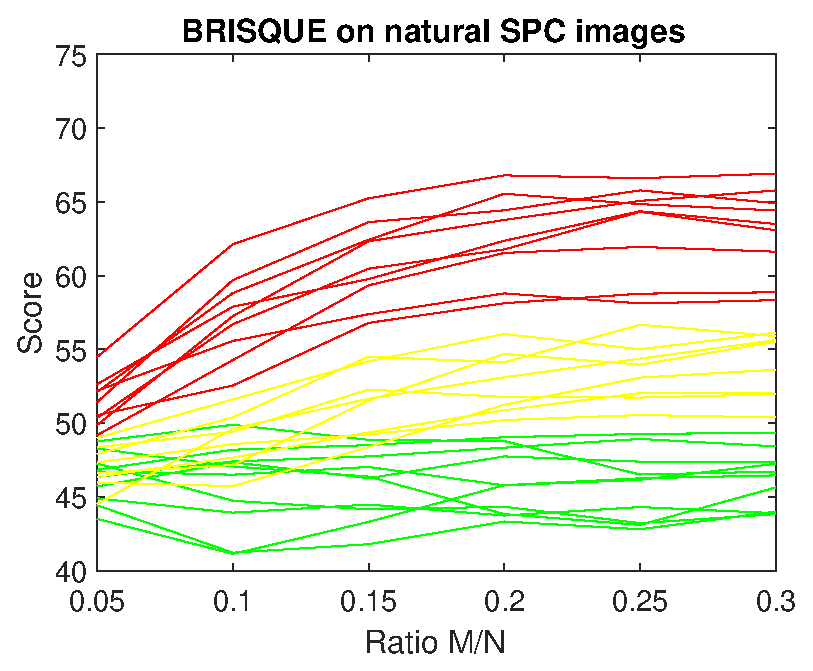
\includegraphics[width = 0.7\linewidth]{result/SPC_NRQA/brisque_spc.eps}
    \caption{BRISQUE score for images reconstructed from the SPC with subsampling ratios from $5\%$ to $30\%$. Each line represent one image and is classified with different colors representing start score at smallest subsampling ratio and general trend when subsampling ratio is increased.}
    \label{fig:brisque_plot}
\end{figure}


As seen in figure~\ref{fig:brisque_plot} each image as been plotted separately, this is because the high variance in the scores and the distinct different trends in the score. Furthermore the images has been classified into three different classes depending on the initial score at 5\% subsampling and the trend when increasing the subsampling ratio\todo{an visually inspecting the images}. The classes has been color coded where:

\begin{itemize}
\item Red means bad score from the first subsampling ratio and a trend line where the score gets worse with more samples.
\item Yellow represent good initial score but the trend line indicates worse image quality when subsampling ratio is increased.
\item Green represent both good initial score and better or stationary score when subsampling ratio is increased. 
\end{itemize}

When studying the BRISQUE score plot in figure~\ref{fig:brisque_plot} from the SPC and comparing to the plot of BRISQUE scores from simulated images in figure~\ref{fig:Brisque_2d} some similarities can be found. The first one is that, the best scores from the SPC has the same score as the simulated images with small or no noise added, which means that the SPC can compare to the benchmark set by the simulated images and thus gives theoretical optimal reconstruction given the measurement matrix and reconstruction algorithm. The second similarity is the trend of the "bad" images which has approximately the same score and trend as the simulated images with larger noise added to the sampled signal. In the last part of this subsection the reconstructed images will first be presented an analyzed followed by a noise analysis to conclude if there is a correlation between noise level and BRISQUE score.\\[0.1in] 


In figure~\ref{fig:good} to \ref{fig:bad} a sample of reconstructed  images are presented from each class with subsampling ratio 30\%. 




\begin{figure}[H]
    \centering
\begin{minipage}[t]{0.245\textwidth}
    
\includegraphics[width=1\textwidth]{result/SPC_NRQA/g64_512_m30.PNG}
    \subcaption{}
    \label{fig:good1}
\end{minipage}
\begin{minipage}[t]{0.245\textwidth}
    
\includegraphics[width = \textwidth]{result/SPC_NRQA/g24_512_m30.PNG}
    \subcaption{}
    \label{fig:good2}
\end{minipage}
\begin{minipage}[t]{0.245\textwidth}
    
\includegraphics[width=1\textwidth]{result/SPC_NRQA/g22_512_m30.PNG}
    \subcaption{}
    \label{fig:good3}
\end{minipage}
\begin{minipage}[t]{0.245\textwidth}
    
\includegraphics[width = \textwidth]{result/SPC_NRQA/g65_512_m30.PNG}
    \subcaption{}
    \label{fig:good4}
\end{minipage}
    \caption{Sample of "good" images corresponding to the green lines in figure~\ref{fig:brisque_plot}.
    (a) and (d) People sitting in the edge of a forest.  (b) Stationary car. (c) Camouflage jackets and a AT-4 anti-tank weapon on the ground.}
    \label{fig:good}
\end{figure}

\begin{figure}[H]
    \centering
\begin{minipage}[t]{0.245\textwidth}
    
\includegraphics[width=1\textwidth]{result/SPC_NRQA/h35_512_m30.PNG}
    \subcaption{}
    \label{fig:half1}
\end{minipage}
\begin{minipage}[t]{0.245\textwidth}
    
\includegraphics[width = \textwidth]{result/SPC_NRQA/h37_512_m30.PNG}
    \subcaption{}
    \label{fig:half2}
\end{minipage}
\begin{minipage}[t]{0.245\textwidth}
    
\includegraphics[width=1\textwidth]{result/SPC_NRQA/h43_512_m30.PNG}
    \subcaption{}
    \label{fig:half3}
\end{minipage}
\begin{minipage}[t]{0.245\textwidth}
    
\includegraphics[width = \textwidth]{result/SPC_NRQA/h62_512_m30.PNG}
    \subcaption{}
    \label{fig:half4}
\end{minipage}
    \caption{Sample of "medium good" images corresponding to the yellow lines in figure~\ref{fig:brisque_plot}.
    (a)  People sitting next to a parking lot. (b) - (d) House facades.}
    \label{fig:half}
\end{figure}

\begin{figure}[H]
    \centering
\begin{minipage}[t]{0.245\textwidth}
    
\includegraphics[width=1\textwidth]{result/SPC_NRQA/b20_512_m30.PNG}
    \subcaption{}
    \label{fig:bad1}
\end{minipage}
\begin{minipage}[t]{0.245\textwidth}
    
\includegraphics[width = \textwidth]{result/SPC_NRQA/b46_512_m30.PNG}
    \subcaption{}
    \label{fig:bad2}
\end{minipage}
\begin{minipage}[t]{0.245\textwidth}
    \includegraphics[width=1\textwidth]{result/SPC_NRQA/b75_512_m30.PNG}
    \subcaption{}
    \label{fig:bad3}
\end{minipage}
\begin{minipage}[t]{0.245\textwidth}
    \includegraphics[width = \textwidth]{result/SPC_NRQA/b79_512_m30.PNG}
    \subcaption{}
    \label{fig:bad4}
\end{minipage}
    \caption{Sample of "bad" images corresponding to the red lines in figure~\ref{fig:brisque_plot}.
    (a)  House facade. (b) Crane (Moving clouds in background). (c) Mjärdevi Center facade (Moving clouds reflection in windows). (d) Mjärdevi Center balcony with people having a break (Moving clouds reflection in windows).}
    \label{fig:bad}
\end{figure}

\todo[inline]{Not analyse, What is the difference?}
Lets analyze the images in figure~\ref{fig:good} to \ref{fig:bad} in order to figure out why the BRISQUE score have such high variance and characteristics when increasing the subsampling ratio. The difference between "good" and "half good" images are very subtle, the intensity and visible noise level is a bit more favorable in the "good" images, but as stated in section~\ref{sec:method_eval} the naturalness of the images differ where the "good" images contains more natural shapes and objects. Between the "good"/"half good" and "bad" images there is a more noticeable difference, the images in the "bad" set has more distinct noise and lower over all intensity which most certainly effect the BRISQUE score. Furthermore some of the "bad" image set had movement when sampled which will definitely increase global noise in the images as concluded in section~\ref{sec:Dynamics_in_scene}.\\[0.1in]

When the images was sampled a correlation between the mean signal strength and reconstruction performance was noticed, this is due to the constant background noise from the SWIR photo diode. In figure~\ref{fig:snr} the mean sampled signal strength was plotted against SNR and signal variance calculated from normalizing the sample signal and background noise. The variance was calculated in the same way as the simulated signals in section\ref{sec:simulated_results}.  Each signal has the same corresponding color code from the BRISQUE plot in figure~\ref{fig:brisque_plot}.
 

\begin{figure}[H]
    \centering
\begin{minipage}[t]{0.495\textwidth}
    \includegraphics[width=1\textwidth]{result/noise/meanV_sigma.eps}
    \subcaption{}
    \label{fig:snr_v_sigma}
\end{minipage}
\begin{minipage}[t]{0.495\textwidth}
    \includegraphics[width = \textwidth]{result/noise/meanV_snr.eps}
    \subcaption{}
    \label{fig:snr_v_SNR}
\end{minipage}
    \caption{Mean sampled signal intensity compared to normalized signal and background noise where each signal has the same corresponding color code from the BRISQUE plot in figure~\ref{fig:brisque_plot}.  (a) Signal intensity against normalized variance from background noise. (b) Signal intensity against SNR from normalized signal and background noise.}
    \label{fig:snr}
\end{figure}

From the two plots in figure~\ref{fig:snr} there are some conclusions that can be made:


\begin{itemize}
\item From both plots in figure~\ref{fig:snr} there is a quite distinct threshold where the signals intensity overcomes the noise level to reconstructed "good" images around 1.2 volt. None of the "good"/"half good" images are below this signal intensity but are mixed over the threshold. 
%The exponential characteristics of the signal to noise ratio given the signal strength means that it should be easy to find a threshold for a given systems background noise.

\item In the plots there are only two signals with higher variance than 0.04 which is the threshold where the the simulated images started to get both worse initial BRISQUE score and worse trend when increasing the subsampling ratio in figure~\ref{fig:Brisque_2d}. This implies that there must be at least one additional factor at play to reduce the image quality in the "bad" set. 


\item There are three red images with almost the same SNR and mean signal intensity as yellow and green images but yields a worse BRISQUE score anyway. This strengthening the statement the there is probably at least on more factor that reduces reconstruction performance.

\item The yellow and green images is mixed for all mean signal strengths which implies that the motive in the images effecting the  BRISQUE score. 

\end{itemize}

\todo[inline]{End klam}


\subsubsection{Luminance Change in scene}
As predicted in section~\ref{sec:Dynamics_in_scene}, dynamics in the scene could result in poor reconstruction performance and an algorithm to suppress this distortion was proposed and tested with good result in the simulated case in section~\ref{sec:dyn_sim}. With a exposure time of just under one minute for the SPC this problem turned out to be constantly present when taking photos at natural scenes outdoors, and the luminace change over time was more complex then the simulated test case. It turned out that the sensor was highly sensitive to luminace change which could not be perceived with the naked eye. This observation should not be unanticipated, the sensor sums up half the scenes light which make the tiniest intensity change for each pixel a large global change. So how did the algorithm hold up for the real application? In figure~\ref{fig:lc_plot} the raw sampled signal is colored red which clearly is not a stationary signal, with the moving average in green and the final improved signal in blue. 

\begin{figure}[H]
\includegraphics[width = 0.8\linewidth]{result/luminance/li.eps}
	\caption{Sampled signal from SPC with light intensity change and the improved moving mean processed signal.}
	\label{fig:lc_plot}
\end{figure}

As can be seen on the moving average plotted, the intensity change is very fast and can change in matter of a split of a second, "k" which is the number of neighboring samples to calculate the average  was set to 75 to match the fast change which corresponds to a window of 50 milliseconds.\\[0.1in]

In figure~\ref{fig:lc_image} a reconstructed image without the method used and one with the method used is displayed.

\begin{figure}[H]
\begin{minipage}[t]{0.49\textwidth}
\includegraphics[width = 1\linewidth]{result/luminance/24_512_m30.PNG}
	\subcaption{}
	\label{lc_bf}
\end{minipage}
\begin{minipage}[t]{0.49\textwidth}
\includegraphics[width = 1\linewidth]{gfx/car/car_m30.png}
	\subcaption{}
	\label{lc_af}
\end{minipage}
	\caption{Reconstructed images, (a) before and (b) after applying moving mean average method.}
	\label{fig:lc_image}
\end{figure}

As can be seen in the figure, the method produces good result, the image reconstructed without the signal processing has a severe global noise due to the non stationary signal and the reconstruction performance significantly significantly lower. This images is actually one of the images captured in good conditions with strong lighting and mild intensity change overall.


\subsubsection{Edge response}
The edge response is used to comparing the sharpness of cameras and lenses. The edge response from the SPC is compared to a state of the art SWIR camera. Two scenes was captured by the SPC and a conventional SWIR camera containing printed sheath of paper with simple tilted shapes on them, see figure~\ref{fig:mtf_target}. 



\begin{figure}[H]
    \centering
    \includegraphics[width=0.8\linewidth]{result/mtf/Target.eps}
    \caption{Printed targets with markings where the edge response measurements was performed}
    \label{fig:mtf_target}
\end{figure}

In the resulting images, edge response measurements was gathered from the specified edges in figure~\ref{fig:mtf_target}, with the result from all edges and both images for respective cameras, a mean and standard deviation is calculated. For the SPC, images reconstructed from 5\% to 30\% was tested in order to see if the subsampling ratio effected the MTF result. In figure~\ref{fig:mtf_target_im} the images from the SWIR camera and SPC are presented.

\begin{figure}[H]
    \centering
\begin{minipage}[t]{0.40\textwidth}
    \includegraphics[width=1\textwidth]{result/mtf/swir2.png}
    \subcaption{}
    \label{fig:mtf_s2}
\end{minipage}
\begin{minipage}[t]{0.40\textwidth}
    \includegraphics[width=1\textwidth]{result/mtf/spc22.png}
    \subcaption{}
    \label{fig:mtf_spc2}
\end{minipage}
\begin{minipage}[t]{0.40\textwidth}
    \includegraphics[width=1\textwidth]{result/mtf/swir1.png}
    \subcaption{}
    \label{fig:mtf_s1}
\end{minipage}
\begin{minipage}[t]{0.40\textwidth}
    \includegraphics[width=1\textwidth]{result/mtf/spc12.png}
    \subcaption{}
    \label{fig:mtf_spc1}
\end{minipage}
    \caption{SPC and state of the art SWIR camera images. (a) and (c) from the conventional SWIR camera and (b) and (c) captured with the SPC.}
    \label{fig:mtf_target_im}
\end{figure}




The edge response is measured in the distance (pixels) required for a edge to rise from $10\%$ to $90\%$ intensity change. In figure~\ref{fig:rise} the result from the experiment in presented. 

\begin{figure}[H]
    \centering
    \includegraphics[width=0.7\linewidth]{result/mtf/Rise10_90.eps}
    \caption{Edge response, distance (pixels) to rise from 10-90\% in average for an edge.}
    \label{fig:rise}
\end{figure}

From the plot in figure~\ref{fig:rise}, a clear difference between the SPC and state of the art SWIR camera can be seen, where the conventional SWIR camera has in average half the distance against the SPC images. Some improvement is seen when the subsample ratio is increased, but the standard deviation is almost constant, meaning that the difference between the state of the art SWIR camera and the SPC, in best case only differ about 0.5 pixels, but in the worst case differ about 1.7 pixels and in average 1.2 pixel.

\subsubsection{Number of measurements}
\label{sec:measurements}
From the theory of compressive sensing the number of measurements needed to reconstruct an image is correlated with the sparsity or compressibility of the image, therefore it is hard to give a good estimate of a subsampling ratio needed to obtain a desired quality of the reconstruction. In addition, using a SPC where noise contaminate the signal and the scene may not be completely stationary, the number of measurements needed will increase in proportion to the noise and the change in the scene. In this subsection the minimum subsampling ratio will be presented followed by how the reconstructed image quality is effected by an increese of subsampling ratio.\\[0.1in]


The minimum number of measurements to reconstruct a image where the motive can be recognized is also effected by the factors described, trying to reconstruct an image under the minimum subsampling ratio results in an image with just noise. A survey of the minimum subsampling ratio was performed on all images captured by the SPC in this thesis, and the result ranged from 2\% to 4\% to obtain a recognizable images, in figure~\ref{fig:minimum_fig} a sample of three images with varying minimum subsambling ratios is displayed.


\begin{figure}[H]
\begin{minipage}[t]{0.32\linewidth} %Car
	\includegraphics[width = 1\linewidth]{result/minimum/24_512_m2.PNG}
	\subcaption{Subsampling ratio 2\%.}
	\label{fig:minimum_car}
\end{minipage}
\begin{minipage}[t]{0.32\linewidth} % Hus
	\includegraphics[width = 1\linewidth]{result/minimum/37_512_m3.PNG}
	\subcaption{Subsampling ratio 3\%.}
	\label{fig:minimum_house}
\end{minipage}
\begin{minipage}[t]{0.32\linewidth} %Sit
	\includegraphics[width = 1\linewidth]{result/minimum/64_512_m3.PNG}
	\subcaption{Subsampling ratio 3\%.}
	\label{fig:minimum_forest}
\end{minipage}
	\caption{Varying minimum subsampling ratios to reconstruct sample images captured by the SPC.}
	\label{fig:minimum_fig}
\end{figure}

In the sample images in figure~\ref{fig:minimum_fig} the minimum subsampling ratio varied between 2\% to 3\%, but as can be seen, this is only the minimum subsampling ratio where the motive is barley recognizable, large structure can be identified but detail is lost. In general a subsampling ratio of 5\% has always succeeded to reconstruct a identifiable image with some fine details, moving along this topic the results from higher subsampling ratios is presented.\\[0.1in]

In figure~\ref{fig:subsampling_ratios} three scenes is reconstructed using different subsample ratios ranging from 5\% to 30\%, for each row the subsampling ratio is increased by 5\% and at the top a reference image from a visual camera is presented. What should be expected is increased image quality with increased subsampling ratio, this result can give an perception of which subsampling ratio is good enough for a given purpose, and as can be seen, the increase of subsampling ratio is not linear proportional to the increase in perceived image quality, just like regular image compression.
     

\begin{figure}[H]
\begin{minipage}[t]{0.3\linewidth} %Car
	\includegraphics[width = 1\linewidth]{gfx/car/car_org.png}
	%\subcaption{Visual camera image.}
	\label{fig:car_org}
\end{minipage}
\begin{minipage}[t]{0.3\linewidth} % Hus
	\includegraphics[width = 1\linewidth]{gfx/hus/hus_org.png}
	\subcaption{Visual camera image.}
	\label{fig:hus_org}
\end{minipage}
\begin{minipage}[t]{0.3\linewidth} %Sit
	\includegraphics[width = 1\linewidth]{gfx/sit/sit_org.png}
	%\subcaption{}
	\label{fig:sit_org}
\end{minipage}
\begin{minipage}[t]{0.3\linewidth} %Car
	\includegraphics[width = 1\linewidth]{gfx/car/car_m5.png}
	%\subcaption{Subsampling ratio 5\%}
	\label{fig:car_m5}
\end{minipage}
\begin{minipage}[t]{0.3\linewidth} % Hus
	\includegraphics[width = 1\linewidth]{gfx/hus/hus_m5.png}
	\subcaption{Subsampling ratio 5\%}
	\label{fig:hus_m5}
\end{minipage}
\begin{minipage}[t]{0.3\linewidth} %Sit
	\includegraphics[width = 1\linewidth]{gfx/sit/sit_m5.png}
	%\subcaption{}
	\label{fig:sit_m5}
\end{minipage}
\begin{minipage}[t]{0.3\linewidth} %Car
	\includegraphics[width = 1\linewidth]{gfx/car/car_m10.png}
	%\subcaption{Subsampling ratio 10\%}
	\label{fig:car_m10}
\end{minipage}
\begin{minipage}[t]{0.3\linewidth} % Hus
	\includegraphics[width = 1\linewidth]{gfx/hus/hus_m10.png}
	\subcaption{Subsampling ratio 10\%}
	\label{fig:hus_m10}
\end{minipage}
\begin{minipage}[t]{0.3\linewidth} %Sit
	\includegraphics[width = 1\linewidth]{gfx/sit/sit_m10.png}
	%\subcaption{}
	\label{fig:sit_m10}
\end{minipage}
\begin{minipage}[t]{0.3\linewidth} %Car
	\includegraphics[width = 1\linewidth]{gfx/car/car_m15.png}
	%\subcaption{Subsampling ratio 15\%}
	\label{fig:car_m15}
\end{minipage}
\begin{minipage}[t]{0.3\linewidth} % Hus
	\includegraphics[width = 1\linewidth]{gfx/hus/hus_m15.png}
	\subcaption{Subsampling ratio 15\%}
	\label{fig:hus_m15}
\end{minipage}
\begin{minipage}[t]{0.3\linewidth} %Sit
	\includegraphics[width = 1\linewidth]{gfx/sit/sit_m15.png}
	%\subcaption{}
	\label{fig:sit_m15}
\end{minipage}
\end{figure}
\begin{figure}[H]
\ContinuedFloat
\begin{minipage}[t]{0.3\linewidth} %Car
	\includegraphics[width = 1\linewidth]{gfx/car/car_m20.png}
	%\subcaption{Subsampling ratio 20\%}
	\label{fig:car_m20}
\end{minipage}
\begin{minipage}[t]{0.3\linewidth} % Hus
	\includegraphics[width = 1\linewidth]{gfx/hus/hus_m20.png}
	\subcaption{Subsampling ratio 20\%}
	\label{fig:hus_m20}
\end{minipage}
\begin{minipage}[t]{0.3\linewidth} %Sit
	\includegraphics[width = 1\linewidth]{gfx/sit/sit_m20.png}
	%\subcaption{}
	\label{fig:sit_m20}
\end{minipage}
\begin{minipage}[t]{0.3\linewidth} %Car
	\includegraphics[width = 1\linewidth]{gfx/car/car_m25.png}
	%
	\label{fig:car_m25}
\end{minipage}
\begin{minipage}[t]{0.3\linewidth} % Hus
	\includegraphics[width = 1\linewidth]{gfx/hus/hus_m25.png}
	\subcaption{Subsampling ratio 25\%}
	\label{fig:hus_m25}
\end{minipage}
\begin{minipage}[t]{0.3\linewidth} %Sit
	\includegraphics[width = 1\linewidth]{gfx/sit/sit_m25.png}
	%\subcaption{}
	\label{fig:sit_m25}
\end{minipage}
\begin{minipage}[t]{0.3\linewidth} %Car
	\includegraphics[width = 1\linewidth]{gfx/car/car_m30.png}
	%\subcaption{Subsampling ratio 30\%}
	\label{fig:car_m30}
\end{minipage}
\begin{minipage}[t]{0.3\linewidth} % Hus
	\includegraphics[width = 1\linewidth]{gfx/hus/hus_m30.png}
	\subcaption{Subsampling ratio 30\%}
	\label{fig:hus_m30}
\end{minipage}
\begin{minipage}[t]{0.3\linewidth} %Sit
	\includegraphics[width = 1\linewidth]{gfx/sit/sit_m30.png}
	%\subcaption{}
	\label{fig:sit_m30}
\end{minipage}
	\label{fig:subsampling_ratios}
	\caption{Reconstructed images captured by the SPC with increasing subsampling ratios. First row showing a reference visual spectrum image followed by SPC images reconstructed with 5\% from top then increased subsampling ratio by 5\% for each row to 30\% on the last row.} 
\end{figure}

The are a few thinks that can be noted in the images in figure~\ref{fig:subsampling_ratios}, 

\begin{itemize}
\item the reconstructed images behave as expected, when the subsample ratio increases the image quality increases. 

\item Already at 5\% subsampling ratio the scene can be properly identified unlike the case in minimal subsamples ratio. The images has some artifacts that can be linked to the reconstruction algorithm, the images looks like the made of small patches.

\item Between 10-15\% the finer details start to appear, like the gap between the panels in the facade, the text on the car and door are getting sharper and the structure of the faces start to appear.

\item As stated before, the image quality does not increase at the same rate as the subsampling ratio, this is most noticeable when increasing the subsampling ratio above 15\%. The improvement after 15\% is not as easy to spot as from the increments before, but they can be found in the details. 
\end{itemize}



 






\section{Discussion}
In this section an analysis and discussion is held to describe how to interpret and explain the result from the evaluation section given the theory in related work.

\subsection{Result} %Varför blev ett visst resultat på ett visst sätt (Objectiva analyser)

\subsection{Method} %Vad jag tycker om det (personliga tankar)

\subsection{Work in a broader context}


\section{Conclusion \& Future Work}
\label{sec:conclusions_and_fw}
%Explicit answers to research questions and a summary of the whole masters thesis.\\[0.1in]
\subsection{Conclusion}
\label{sec:conclusion}

In this thesis a complete compressive imaging SWIR SPC architecture was implemented and evaluated. The aim was to find out which image quality could be achieved in natural images captured in daylight. The results produced in thesis both presented evaluation from simulated images and images captured by the SPC to show how the chosen sampling method and reconstruction algorithm performed and how the whole architecture performed in unison.\\[0.1in]

The sampling strategy using the structural random matrices method with sequency ordered Walsh Hadamard measurement matrix solved the problems of scaling the reconstructed images to high definition photos and enabled the image resolution $512 \times 512$ pixels in this thesis, the same resolution as the state of the art reference SWIR camera.\\[0.1in]

The total variation solver TVAL3 was used as reconstruction algorithm  which took advantage of SRM with FWHT to reconstruct the images fast and with good preservation of edges. Using the chosen sampling and reconstruction method could potentially make for a lightweight sampling and reconstruction procedure with few variables stored in memory and calculations made in real time.\\[0.1in]

Feeding the measurement matrices to the DMD through a HDMI cable and video software was an easy method to start with. The first set of measurements was performed with low frame rate and blank frames for control. But when maximizing the frame rate the risk of duplicate or frame drops increased which made it hard to par each measurement to the correct measurement matrix. This method need to be replaced for more control and faster sampling rates.

In post processing an algorithm to correct the signal effected by luminance change was implemented, this algorithm showed to be of utmost importance to this thesis. Long exposure time in natural scenes always gave a significant DC change in the sampled signal which should be stationary. Result showed in both simulation of luminance change and in real scenes a significant improvement of image quality when using this method and the analysis indicate that the algorithm may be relevant even if the exposure time gets reduced to near a second.\\[0.1in]

The resulting images produced by the SPC shows that high quality and high resolution images can be acquired in natural daylight scenes. In good conditions with enough intensity to overcome the sensors background noise and relatively stationary scenes, detailed images where even people could be identified, could be reproduced. Given the result and further work and improvement of the hardware, compressive imaging and the SPC architecture have potential of real world applications.\\[0.1in]

The resulting reconstructed images from both simulations and the SPC was evaluated with a range of methods. When a reference image was available, standard image evaluation techniques, PSNR and SSIM was used. In the subsampling range 5-30\% as was used through out the thesis showed that image quality increased with increasing subsampling ratio but stagnated around a subsampling ratio between 15-20\%. The BRISQUE no reference image quality assessment algorithm indexed based on statistics of "naturalness" in the images and it could be seen that the SPC could get the same results as the best in the simulations indicating that the sampling and reconstruction is the main source of image degradiation and that the SPC hardware in the right conditions do not effects the resulting image quality negatively.\\[0.1in] 

The edge response algorithm calculates the sharpness of the image and therefore comparison between cameras and image processing methods is easily performed. This evaluation showed that the reference SWIR camera performs a bit better than the SPC. Because the SWIR SPC is a completely different camera than a conventional camera and has a different purpose and application than a regular camera a good evaluation is also to present the produced images to get a subjective view of the quality and what is good enough.\\[0.1in]


In this last paragraph a summarize of the whole thesis is made by answering the research questions:


\begin{itemize}
    \item The image quality of the produced images can be evaluated with the same methods used when evaluating a regular camera. But in the case of the SPC the sampling matrix and reconstruction algorithm can be evaluated independently of the camera as well.
    
    \item The state of the art method to capture and reconstruct images using a SPC architecture is to sample all the measurement matrices as fast as possible using structurally random matrices and fast transforms in the reconstruction algorithm.
    
    \item The image quality achieved using state of the art methods applied to the SPC is high resolution images with good enough quality to be used in real world applications. 
\end{itemize}







\subsection{Future work}
This thesis shows that there is possible to use the SPC architecture to capture and reconstruct natural scenes in daylight, but for the technology to be used in a realistic application some improvements can be made. And I think the most crucial problems could be "bought out" by more sophisticated hardware.\\[0.1in]

As identified multiple times in this thesis, the largest contributor to decreased image quality is exposure time and noise. The exposure time can be decreased by a faster DMD, today there exist a DMD:s with 8 times the maximum pattern rate of the DMD used in this thesis (which was operated at half the maximum speed), which would enable an exposure time of 1.125 seconds at 10\% subsampling ratio. This upgrade would however require a new approach to feeding the measurements matrices to the DMD because of the limitations of the HDMI cables transfer speed.\\[0.1in]

Ether if a new transfer approach is implemented or not, a more sophisticated method of generating each measurement matrix should be implemented, the current method of generating all  measurement matrices offline to a video file and then playbacked by a third party video player which has a limitation of FPS but also a reliability problem. The software was not designed to necessarily show every frame in the video file, which is a problem where each measurement needs to be paired with the correct measurement matrix. My suggestion would be a program which would calculate all matrices at start up and upload them to video memory ready for to display at the DMD. This solution would also be more agile where subsampling ratio, which type of measurement matrix and exposure time could easily be adjusted prior to sampling.\\[0.1in]

The second hardware upgrade, to reduce noise, would be to replace the photo diode used in this thesis to a more appropriate sensor for the application. The new sensor should have less background noise and the surface area of the doid should be analyzed to match the rest of the architecture to maximize the incoming light onto the sensor through the focusing lens. This upgrade could also unlock the true potential of the SWIR spectrum where images could be captured in dark environments illuminated by the moon, stars and night glow.\\[0.1in]

New research shows promising results by adding a second sensor which measures the intensity of the mirrors representing zero or turned away from the sensor and being dumped in the current architecture. The compliment of each unique measurement matrix could also be seen as a unique measurement matrix and thus more information is collected in each measurement and thus reduce the subsampling ratio needed to reconstruct a corresponding single sensor image.\cite{article:nature_dual_sensor}\\[0.1in]

The last future work proposition will not increase image quality but would simplify research or usage and time consumption taking pictures with the SPC. The second and third most time consuming task after exposure time is the complexity of sampling the scene and the reconstruction algorithm in the post process. A fully integrated capturing and reconstruction chain with a gpu accelerated reconstruction algorithm should ease the work and save a lot of time for the user. 
 


%\part*{Appendix}
%\appendix
%\include{detaljer}
\include{rtthesis-doc}
\clearemptydoublepage
\backmatter

\bibliography{IEEEfull,myrefs}

\printindex

\end{document}